\begin{figure}[!htbp]
  \centering
  \begin{subfigure}[b]{0.47\linewidth}
      \centering
      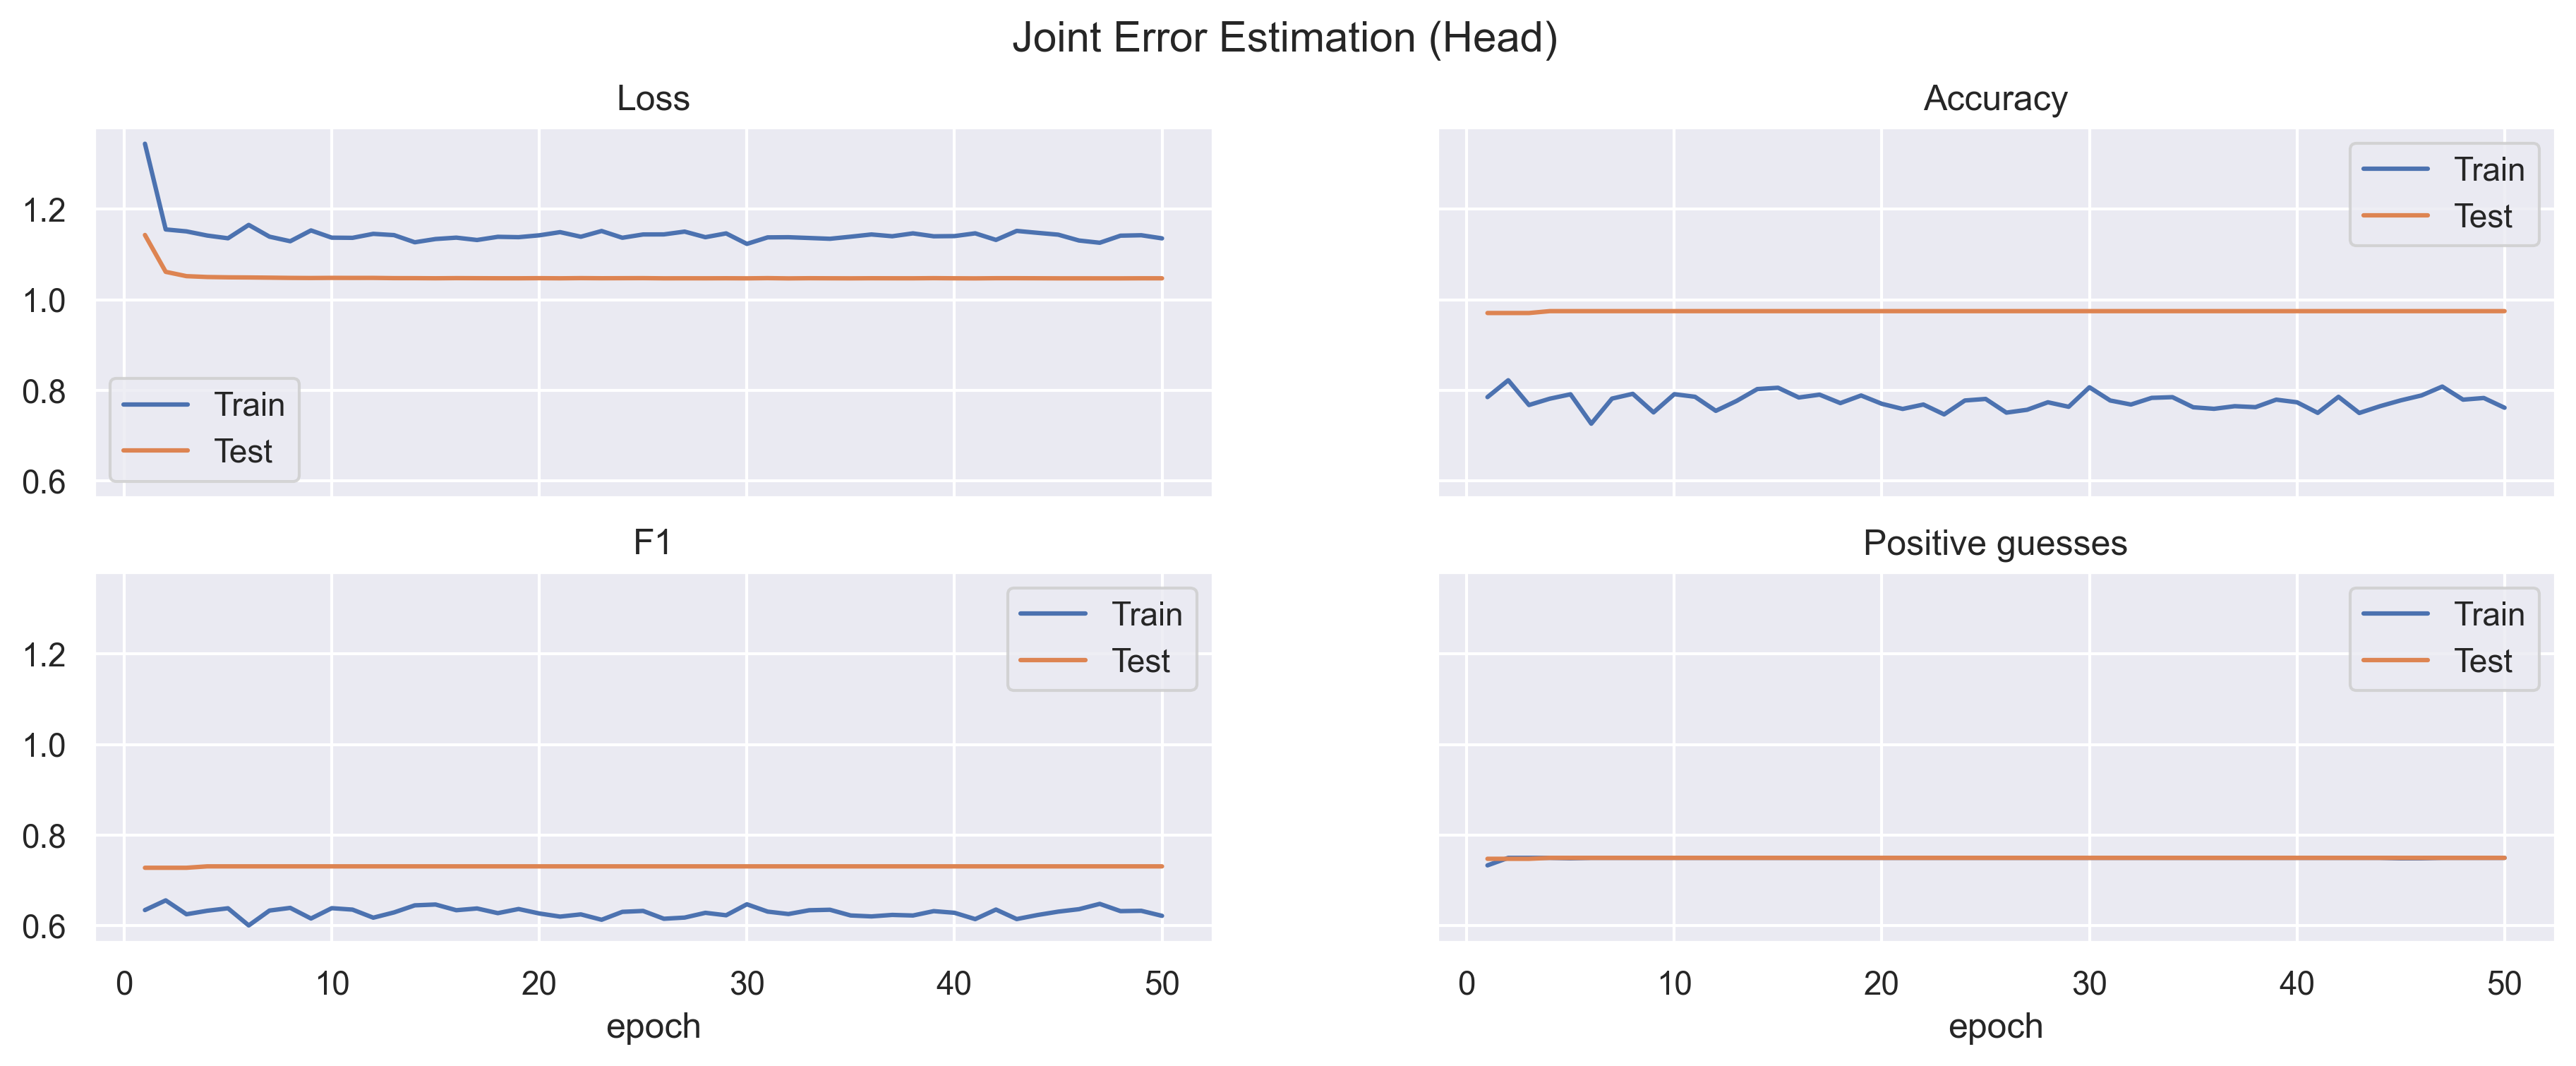
\includegraphics[width=\textwidth]{figures/Results/v1/jt/Head_ErrorEstimation.png}
      \caption{Head Error Estimation}
      \label{fig:v1_head_jt_ee}
  \end{subfigure}
  \hfill
  \begin{subfigure}[b]{0.47\linewidth}
      \centering
      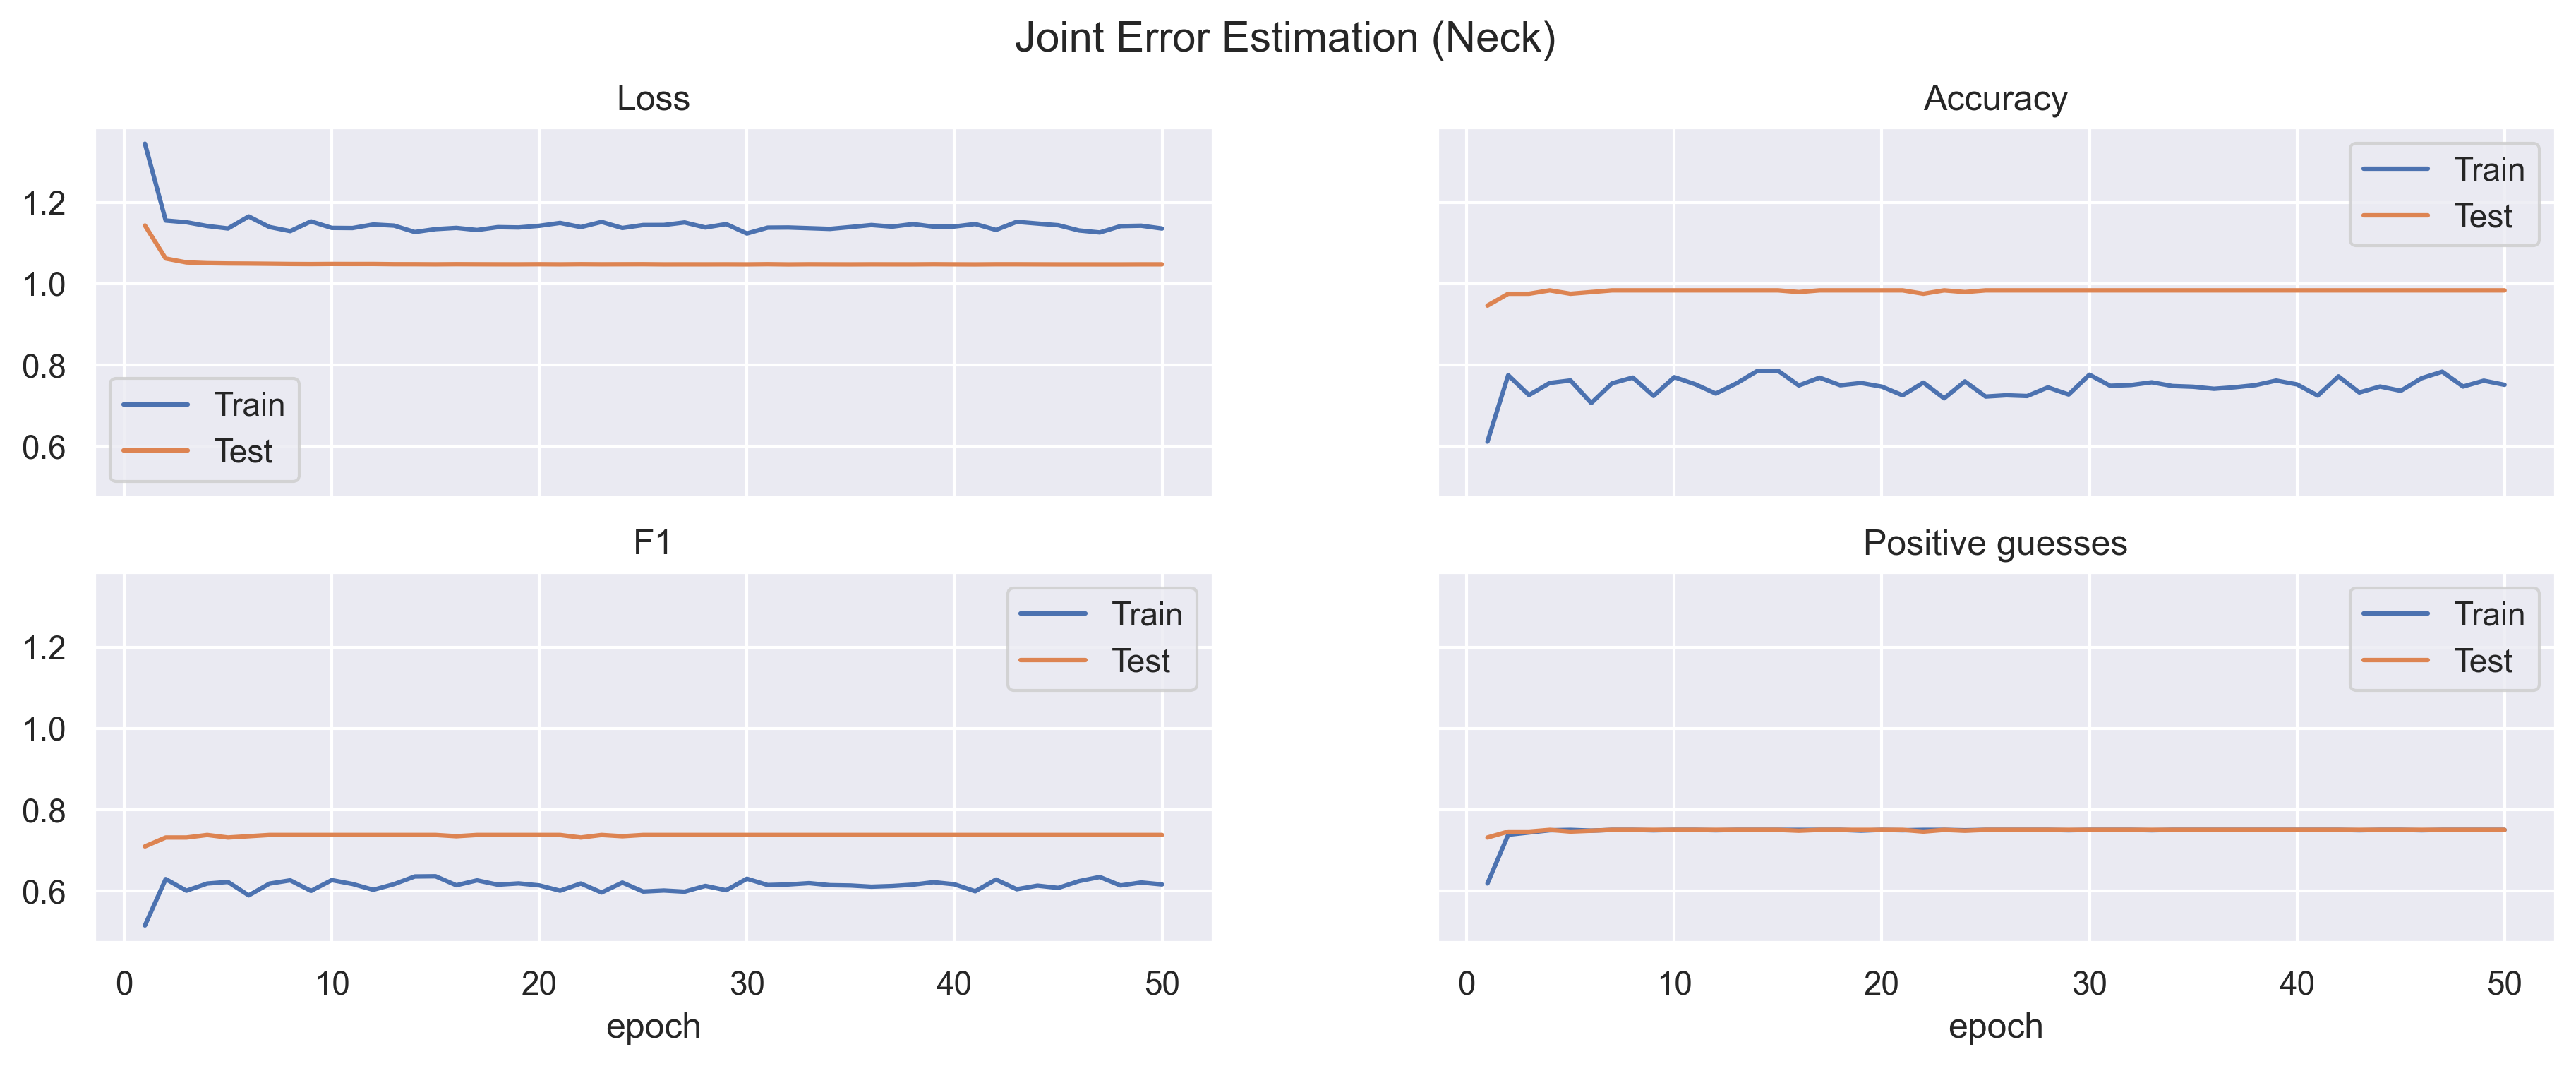
\includegraphics[width=\textwidth]{figures/Results/v1/jt/Neck_ErrorEstimation.png}
      \caption{Neck Error Estimation}
      \label{fig:v1_neck_jt_ee}
  \end{subfigure}
  \hfill
  \begin{subfigure}[b]{0.47\linewidth}
      \centering
      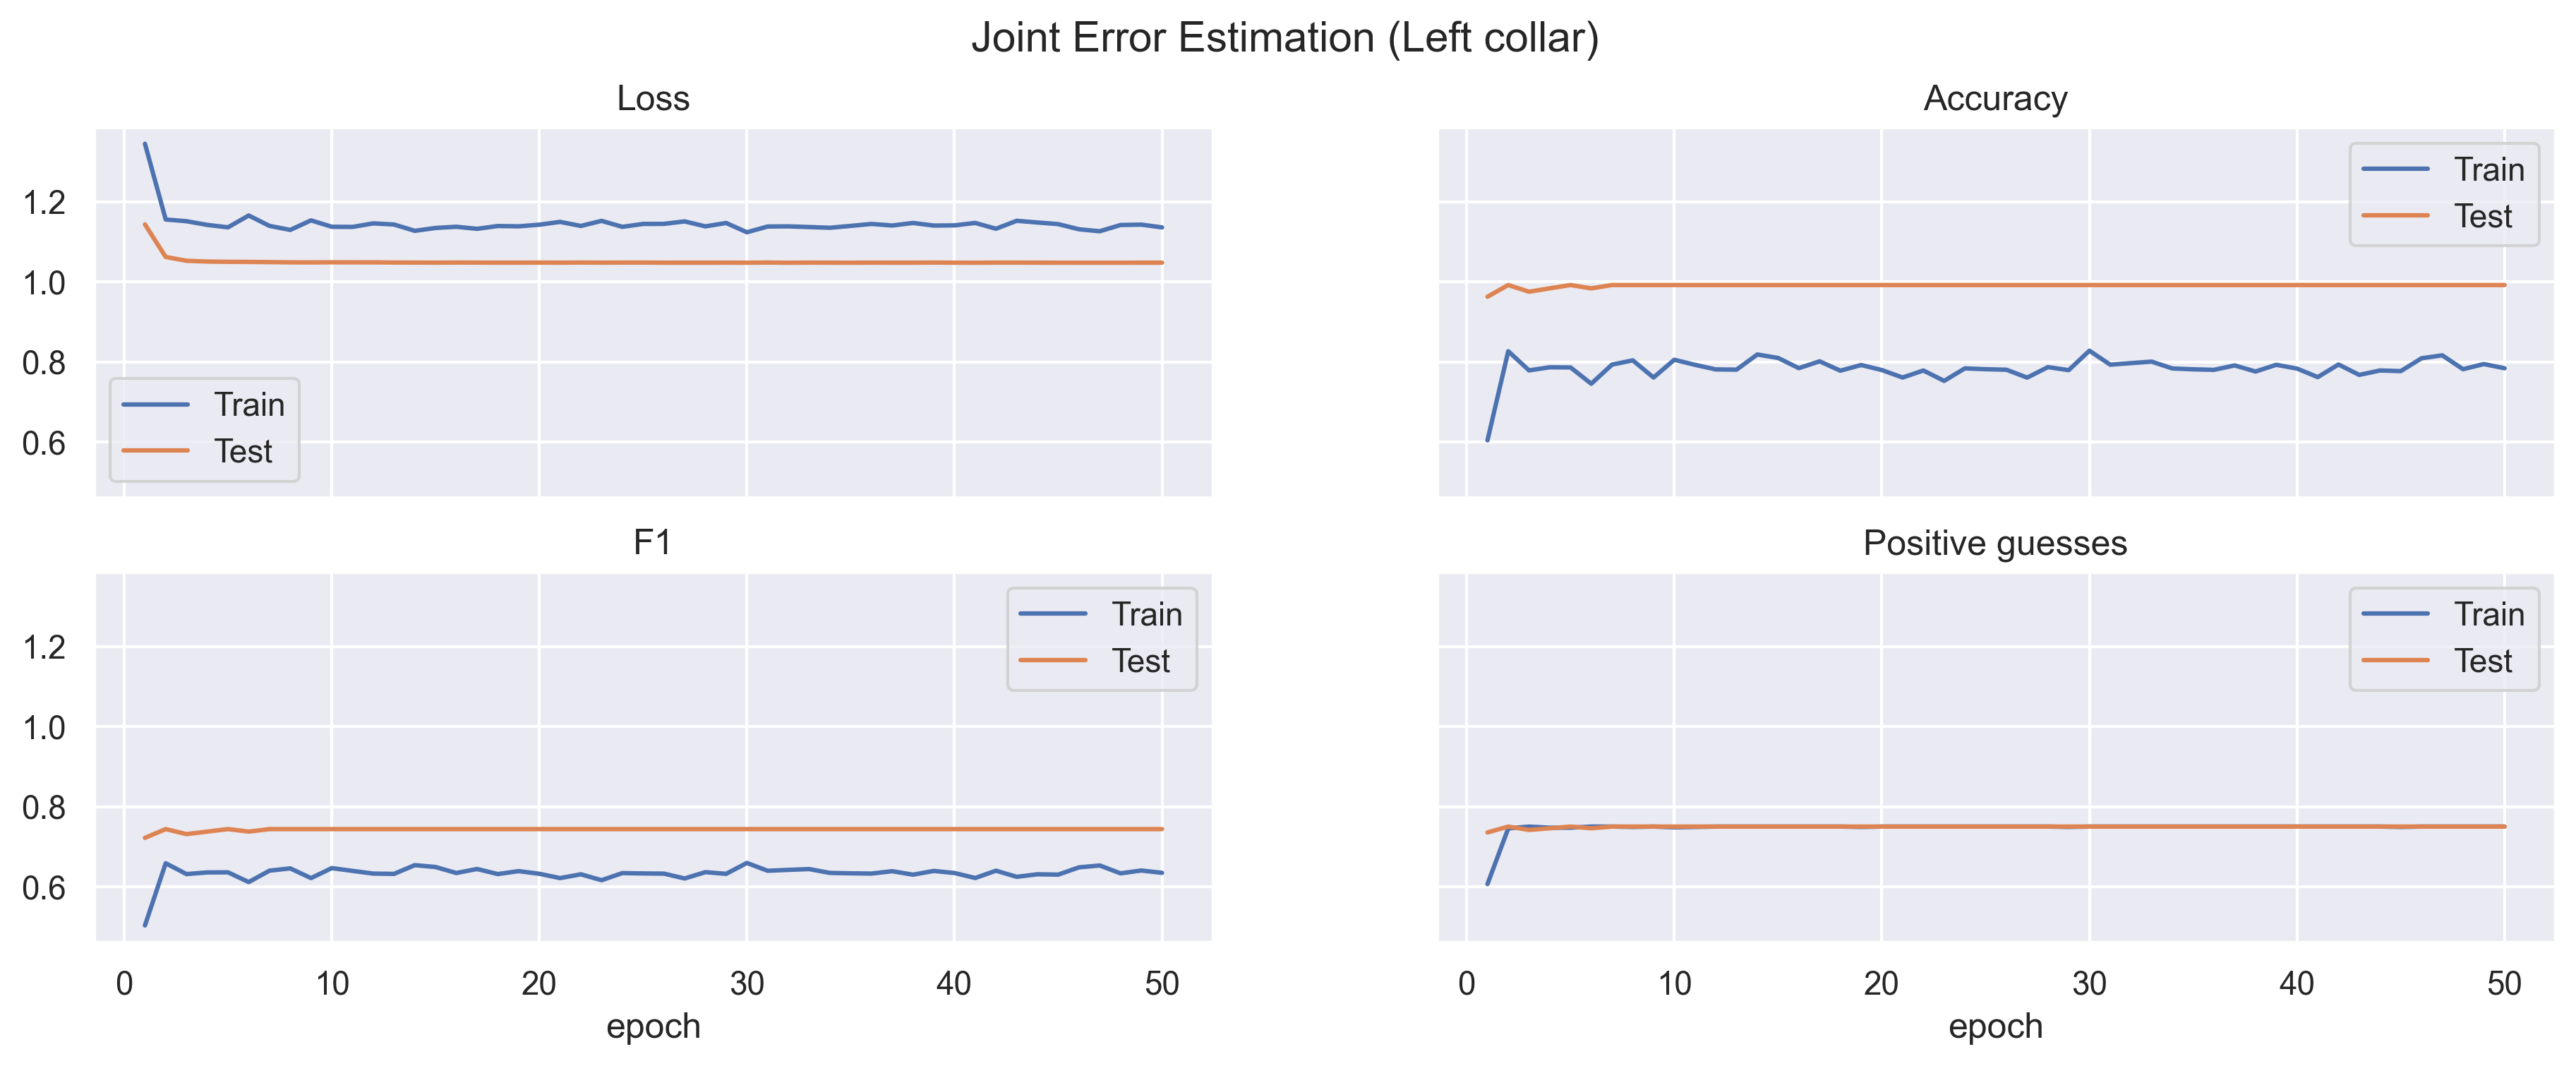
\includegraphics[width=\textwidth]{figures/Results/v1/jt/Left collar_ErrorEstimation.png}
      \caption{Left Collar Error Estimation}
      \label{fig:v1_leco_jt_ee}
  \end{subfigure}
  \hfill
  \begin{subfigure}[b]{0.47\linewidth}
      \centering
      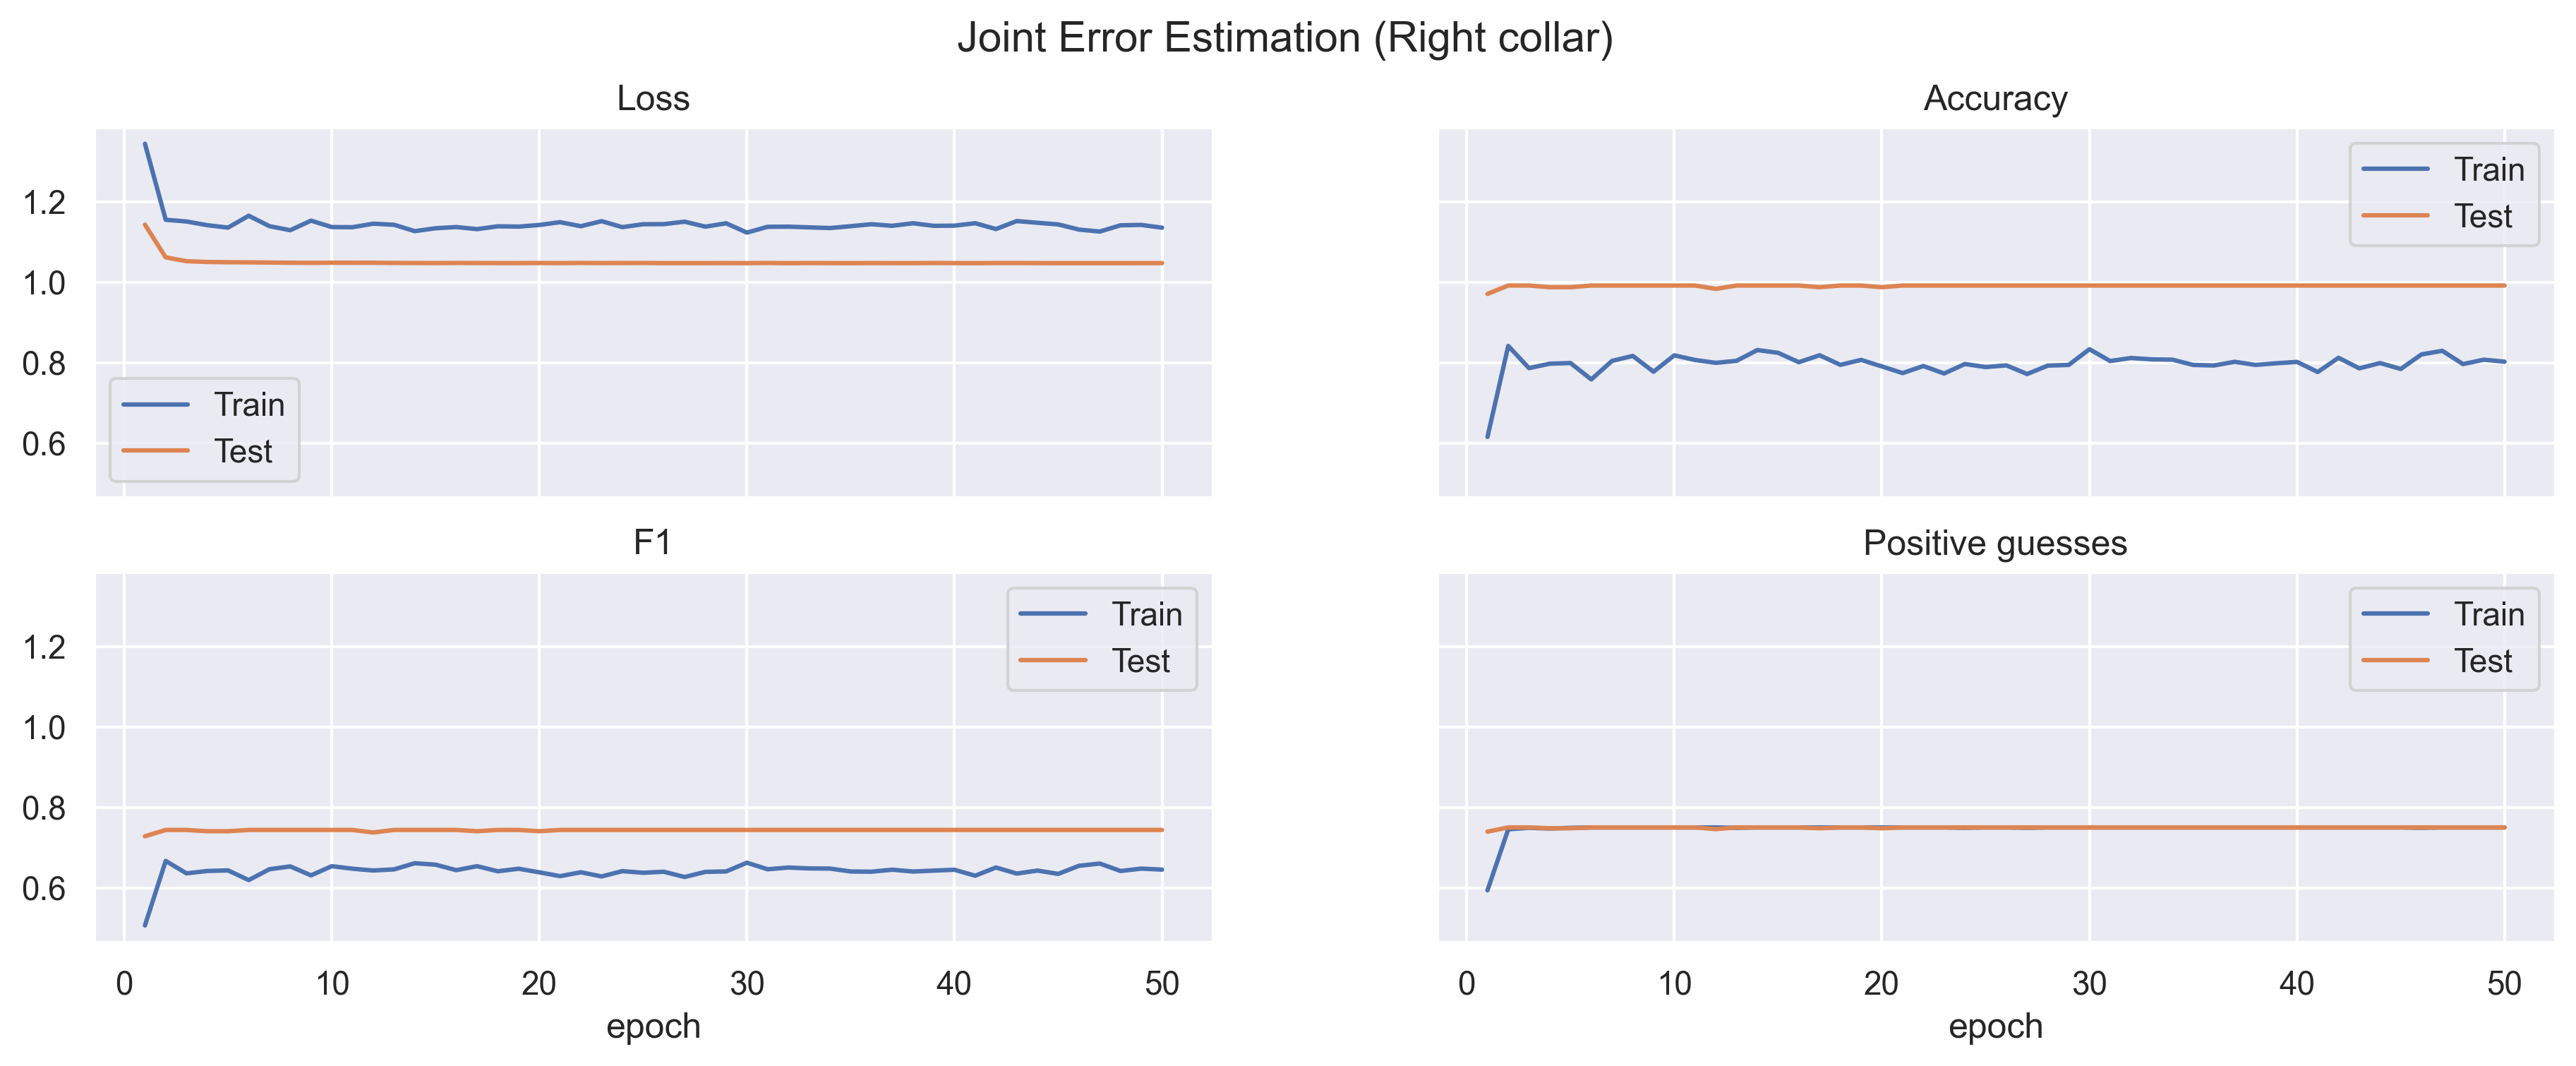
\includegraphics[width=\textwidth]{figures/Results/v1/jt/Right collar_ErrorEstimation.png}
      \caption{Right Collar Error Estimation}
      \label{fig:v1_rico_jt_ee}
  \end{subfigure}
\end{figure}


\begin{figure}[!htbp]
  \centering
  \begin{subfigure}[b]{0.47\linewidth}
      \centering
      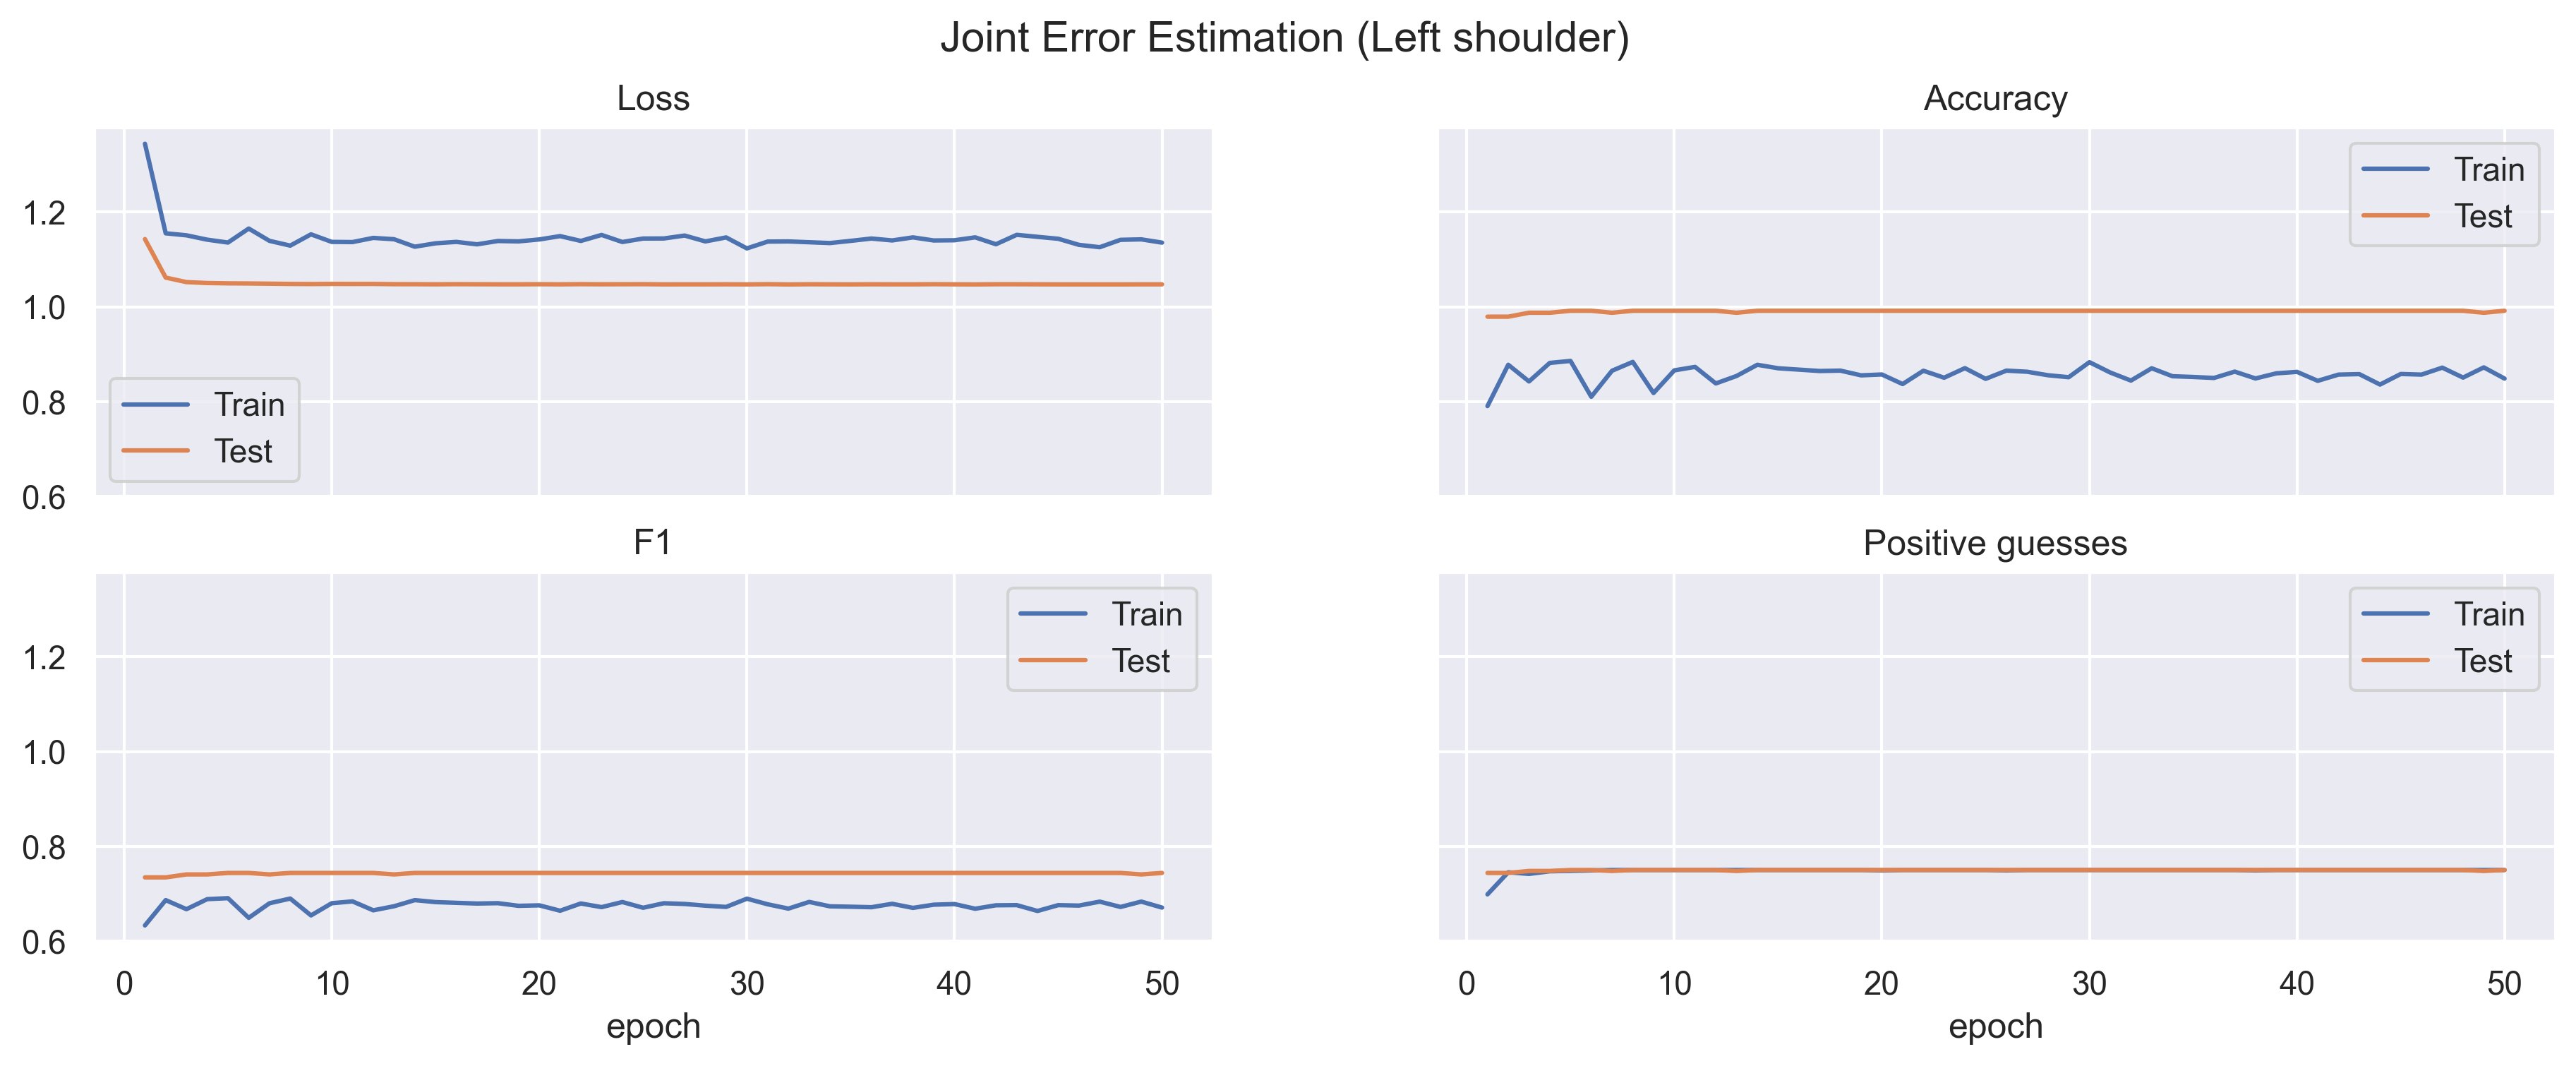
\includegraphics[width=\textwidth]{figures/Results/v1/jt/Left shoulder_ErrorEstimation.png}
      \caption{Left Shoulder Error Estimation}
      \label{fig:v1_lesh_jt_ee}
  \end{subfigure}
  \hfill
  \begin{subfigure}[b]{0.47\linewidth}
      \centering
      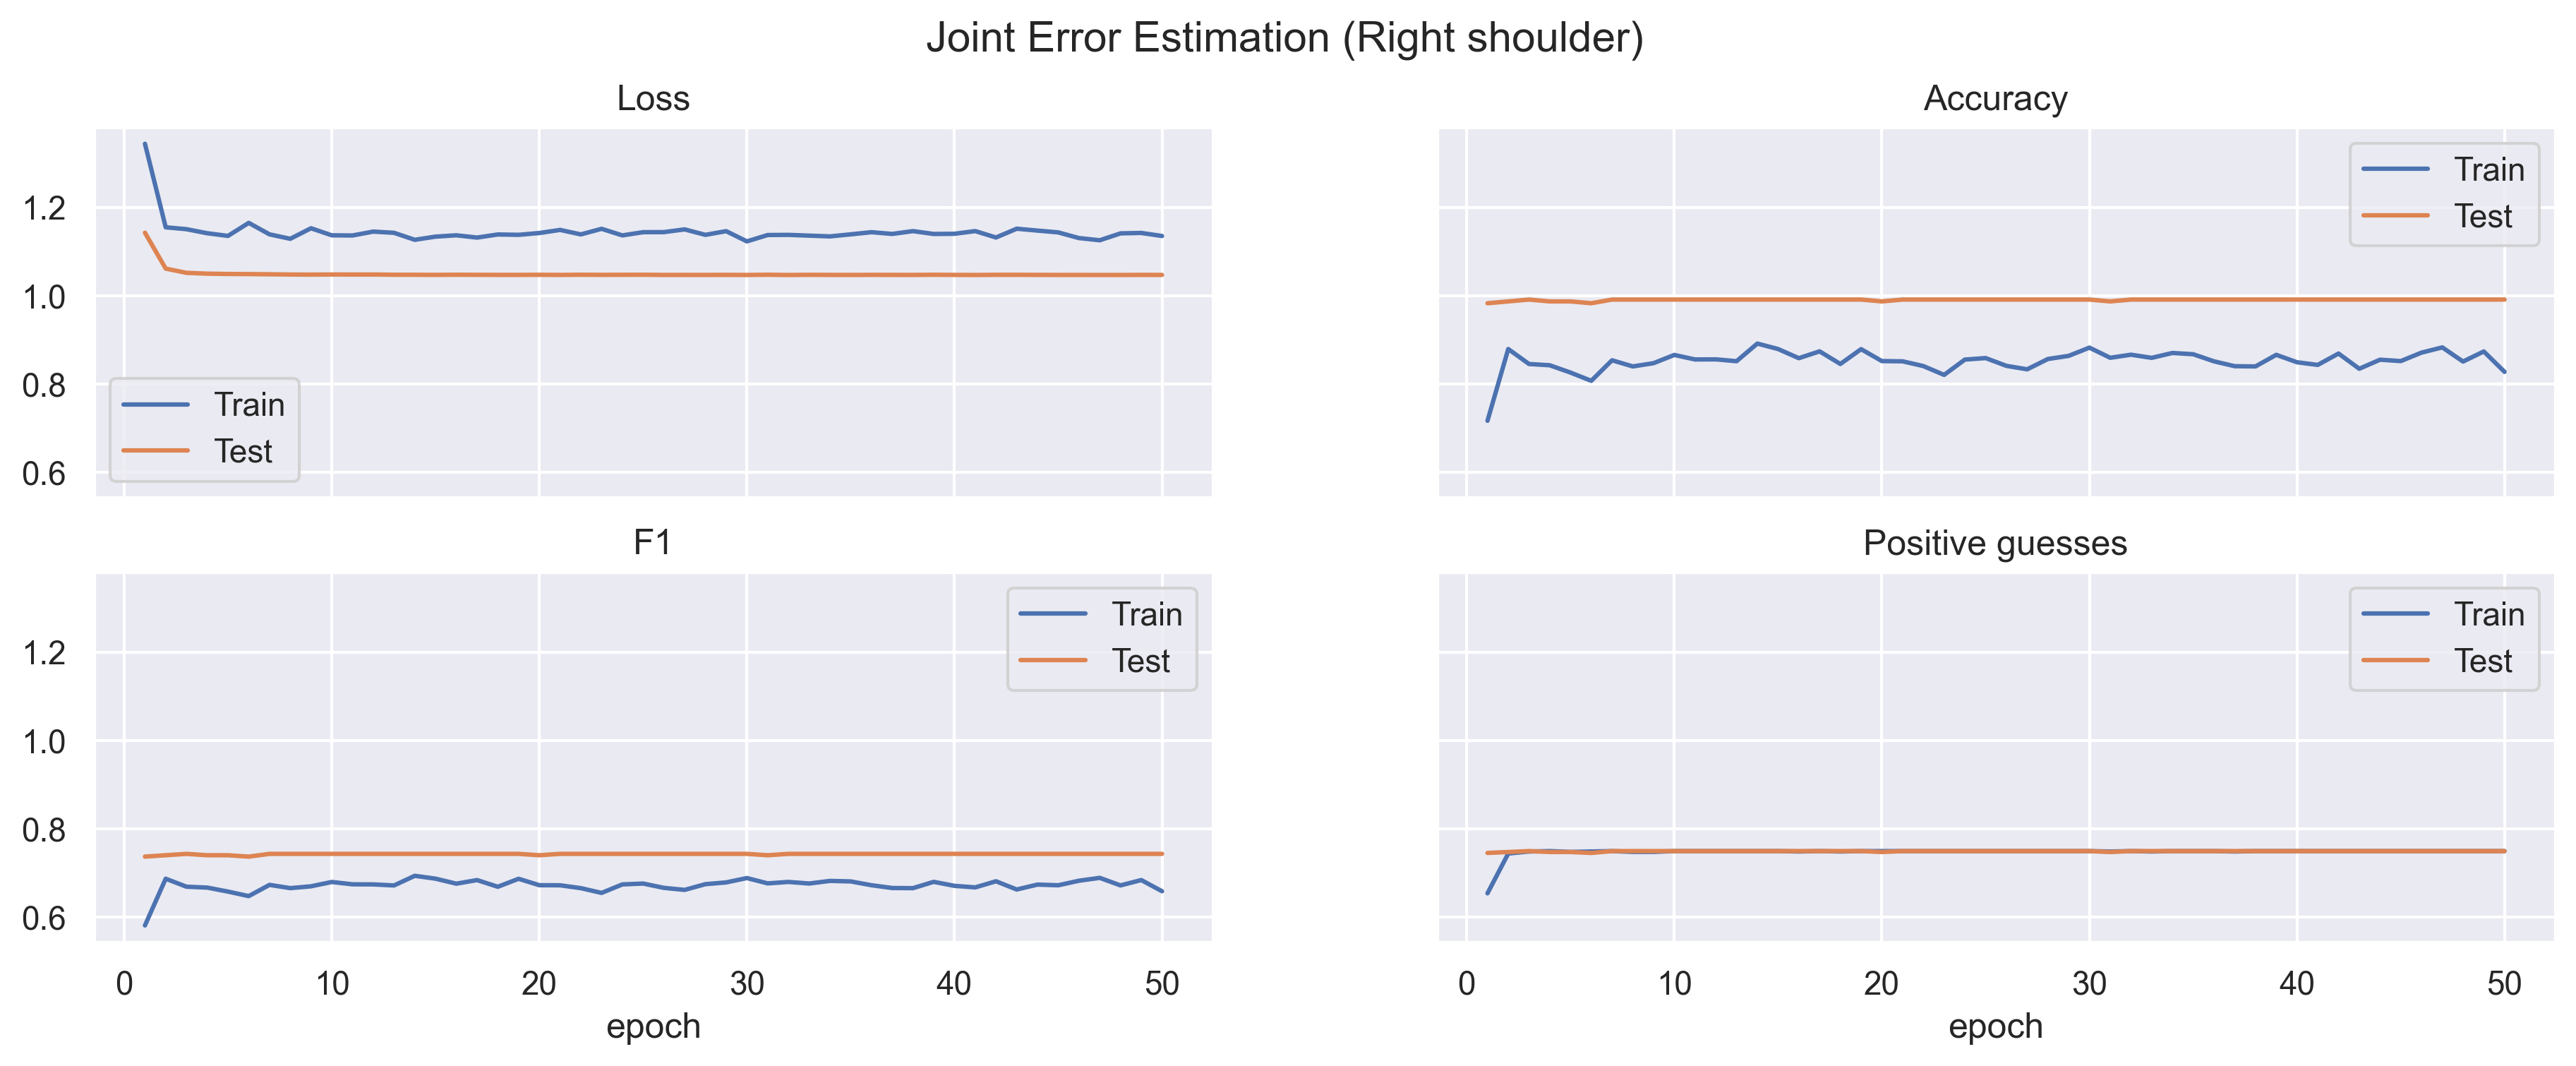
\includegraphics[width=\textwidth]{figures/Results/v1/jt/Right shoulder_ErrorEstimation.png}
      \caption{Right Shoulder Error Estimation}
      \label{fig:v1_rish_jt_ee}
  \end{subfigure}
  \hfill
  \begin{subfigure}[b]{0.47\linewidth}
      \centering
      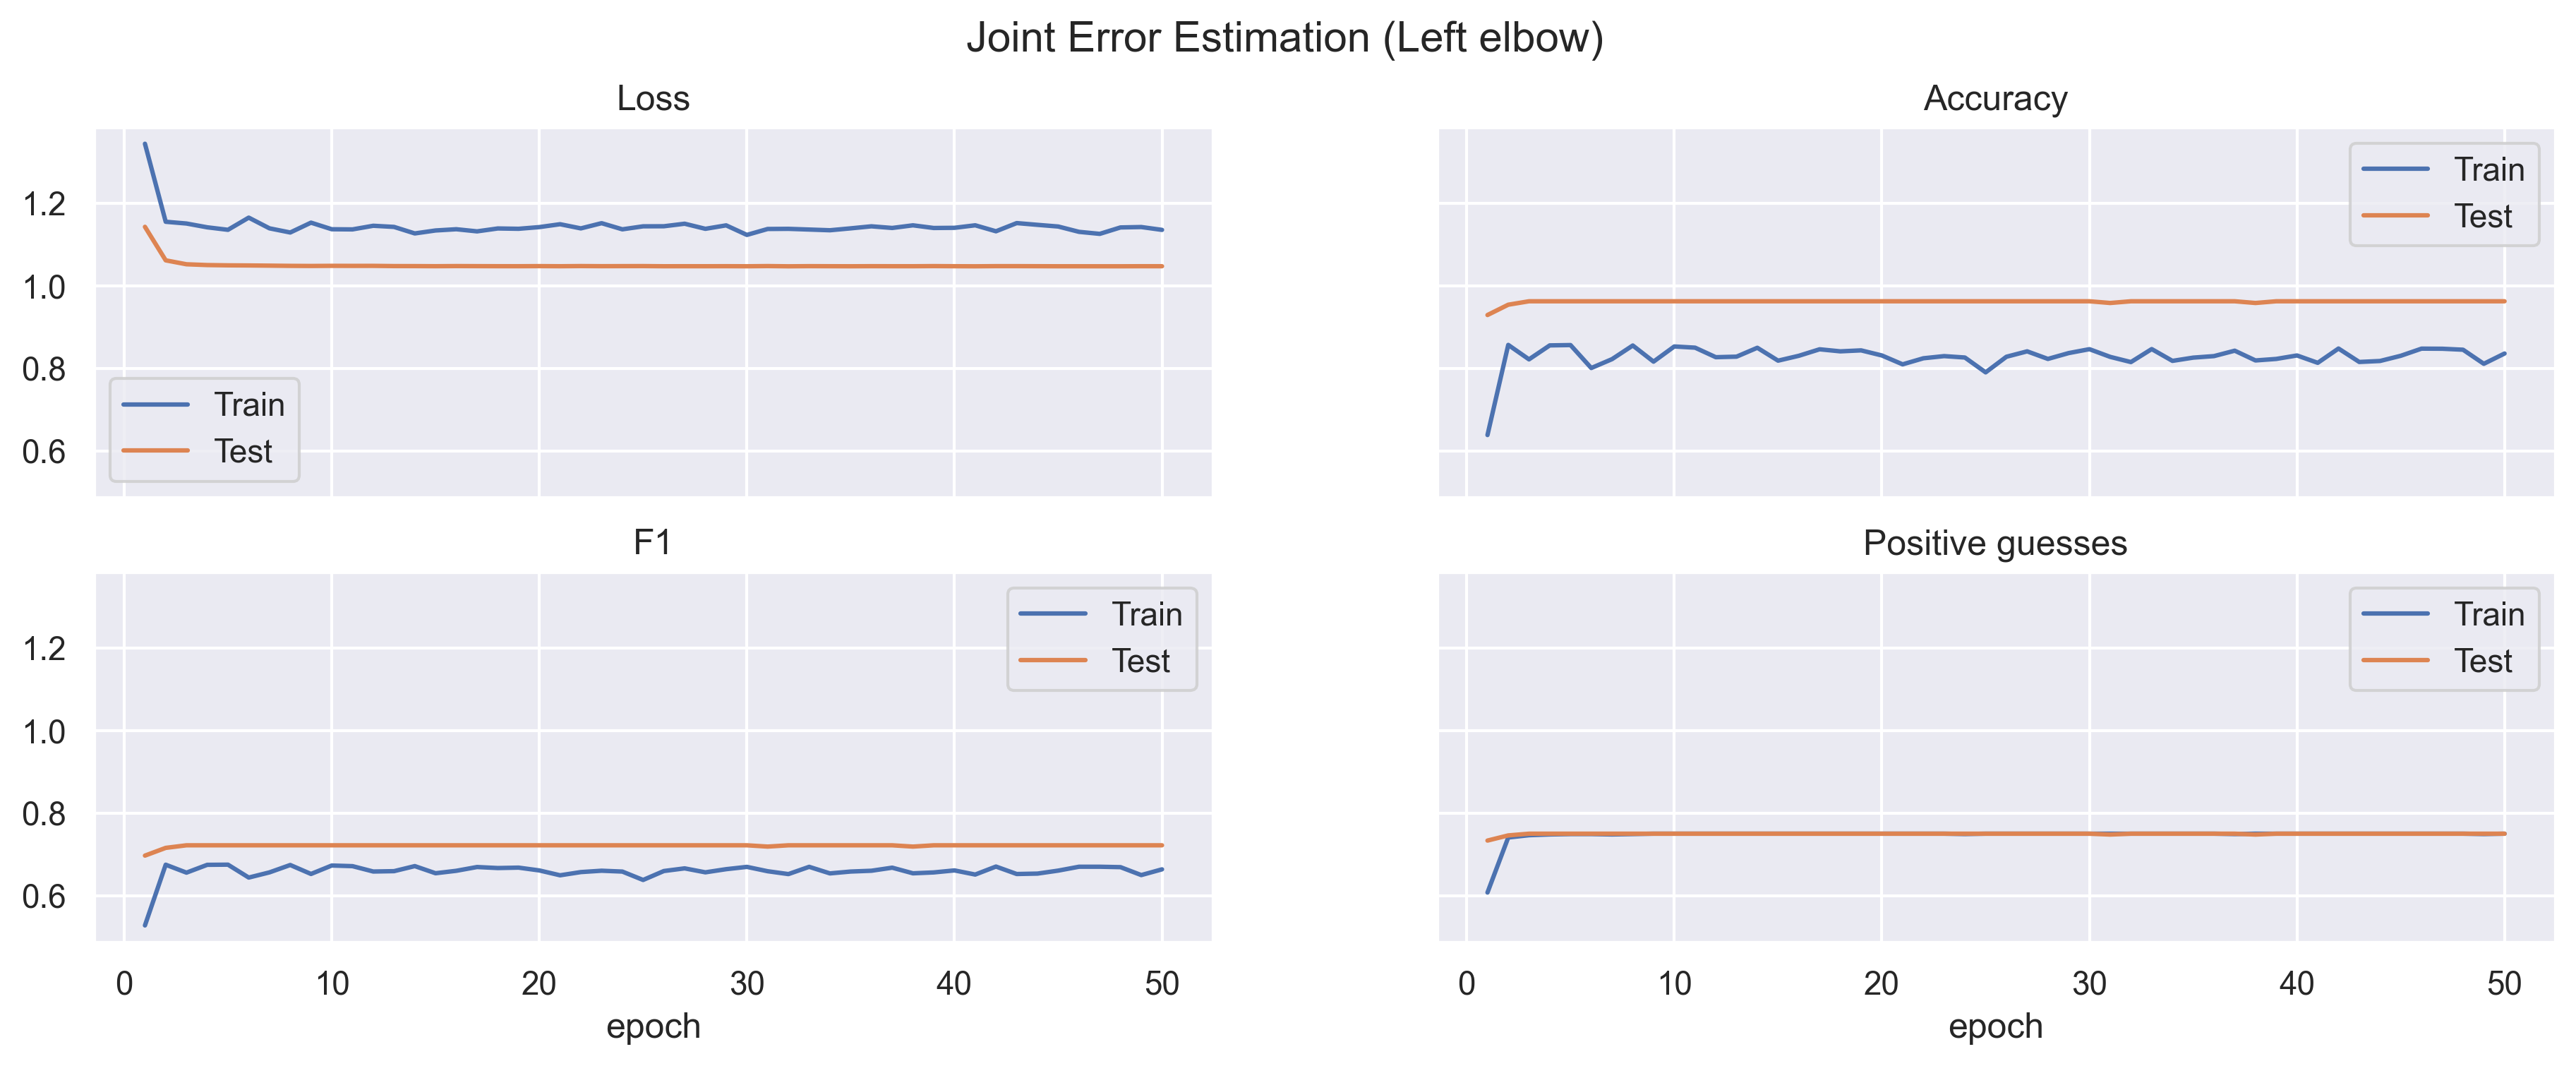
\includegraphics[width=\textwidth]{figures/Results/v1/jt/Left ebpow_ErrorEstimation.png}
      \caption{Left Elbow Error Estimation}
      \label{fig:v1_leel_jt_ee}
  \end{subfigure}
  \hfill
  \begin{subfigure}[b]{0.47\linewidth}
      \centering
      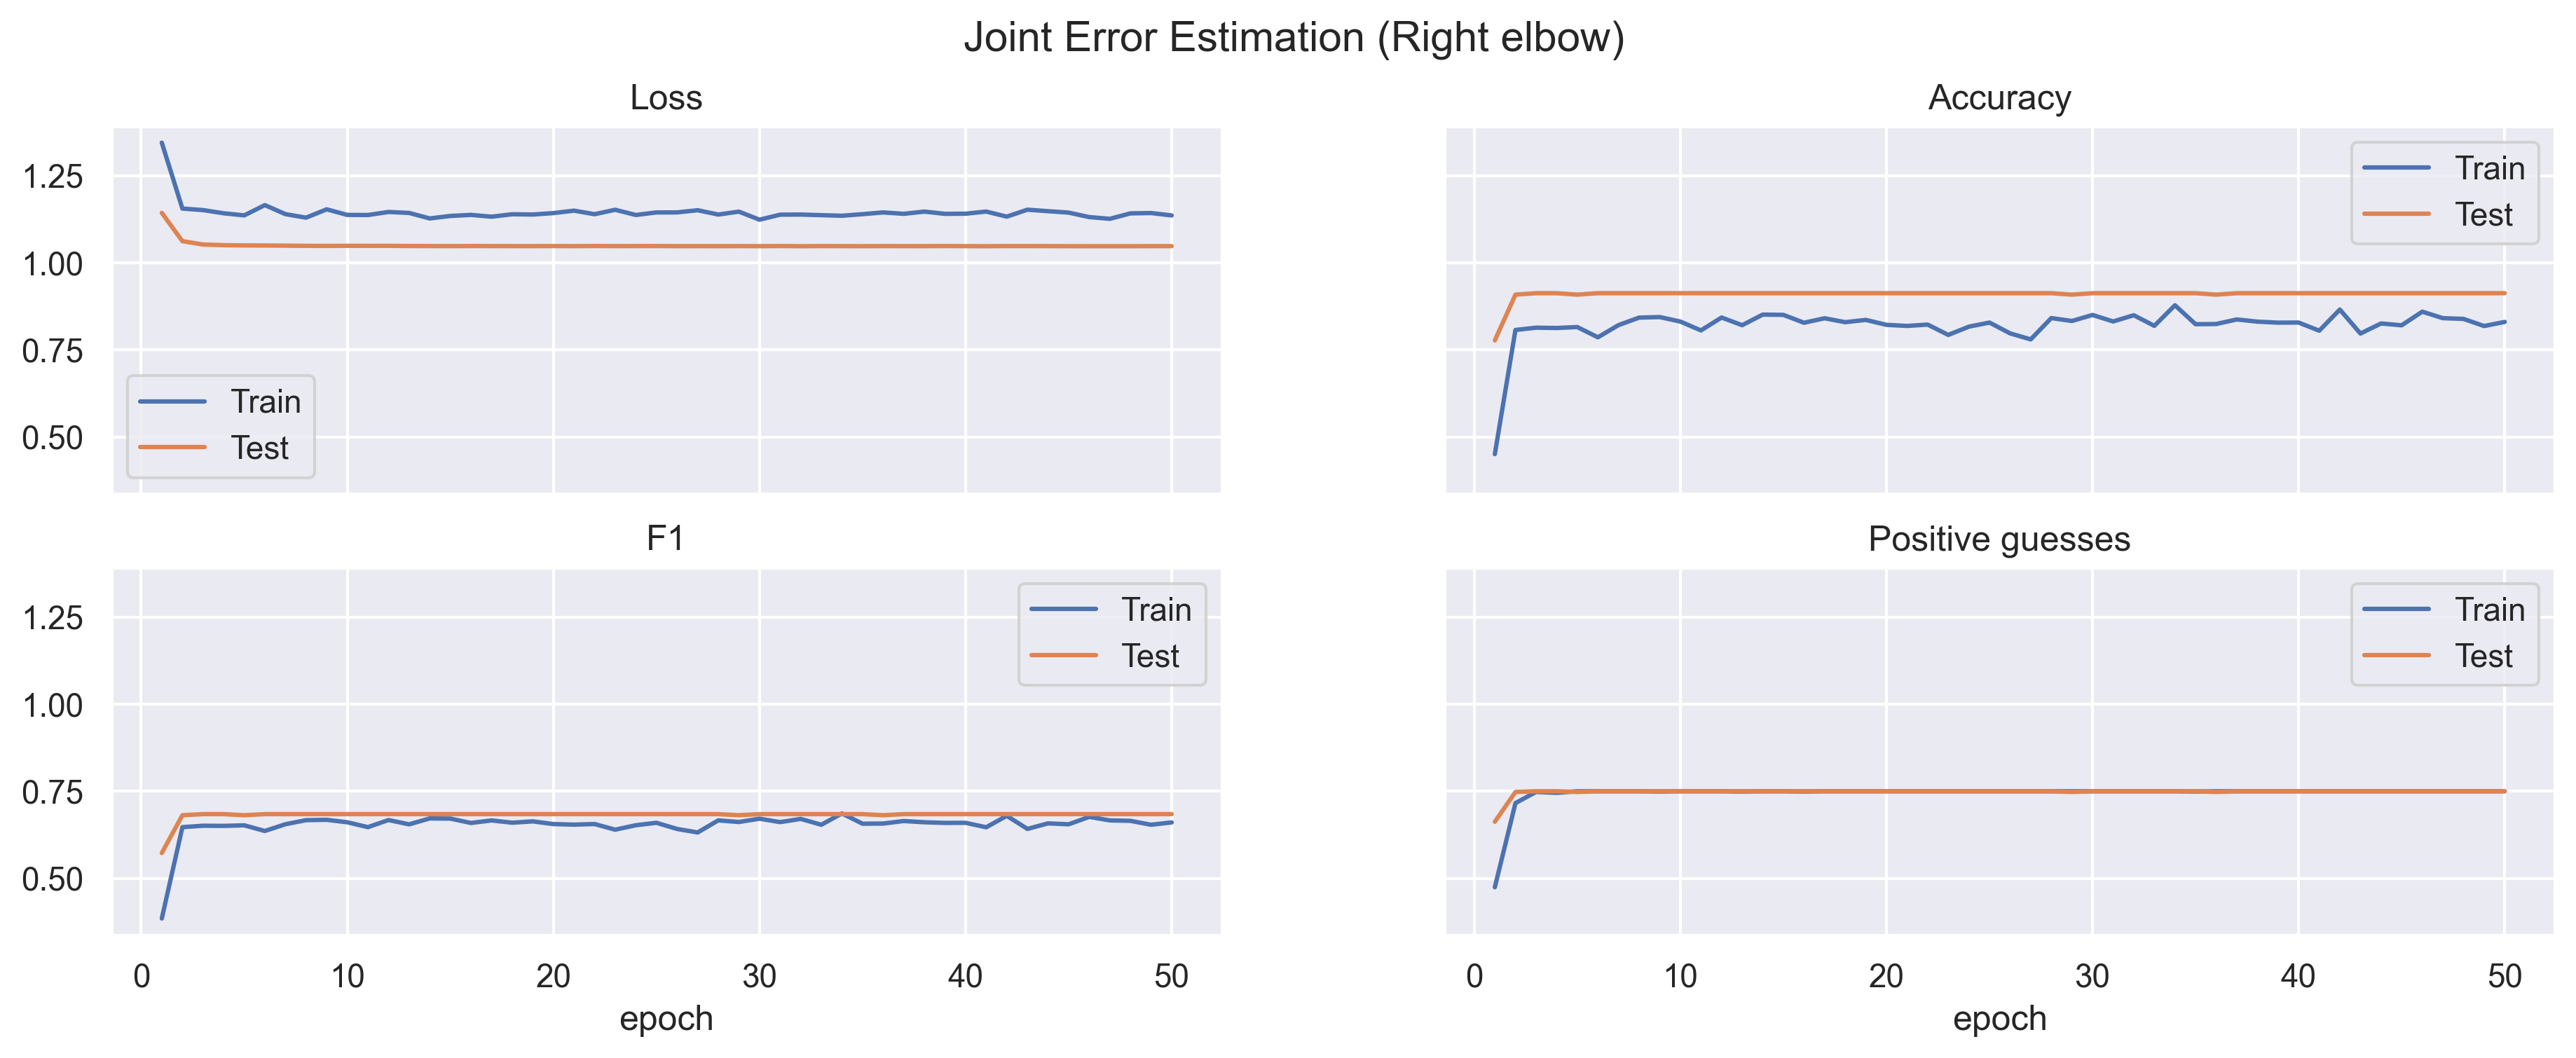
\includegraphics[width=\textwidth]{figures/Results/v1/jt/Right elbow_ErrorEstimation.png}
      \caption{Right Elbow Error Estimation}
      \label{fig:v1_reel_jt_ee}
  \end{subfigure}
\end{figure}


\begin{figure}[!htbp]
  \centering
  \begin{subfigure}[b]{0.47\linewidth}
      \centering
      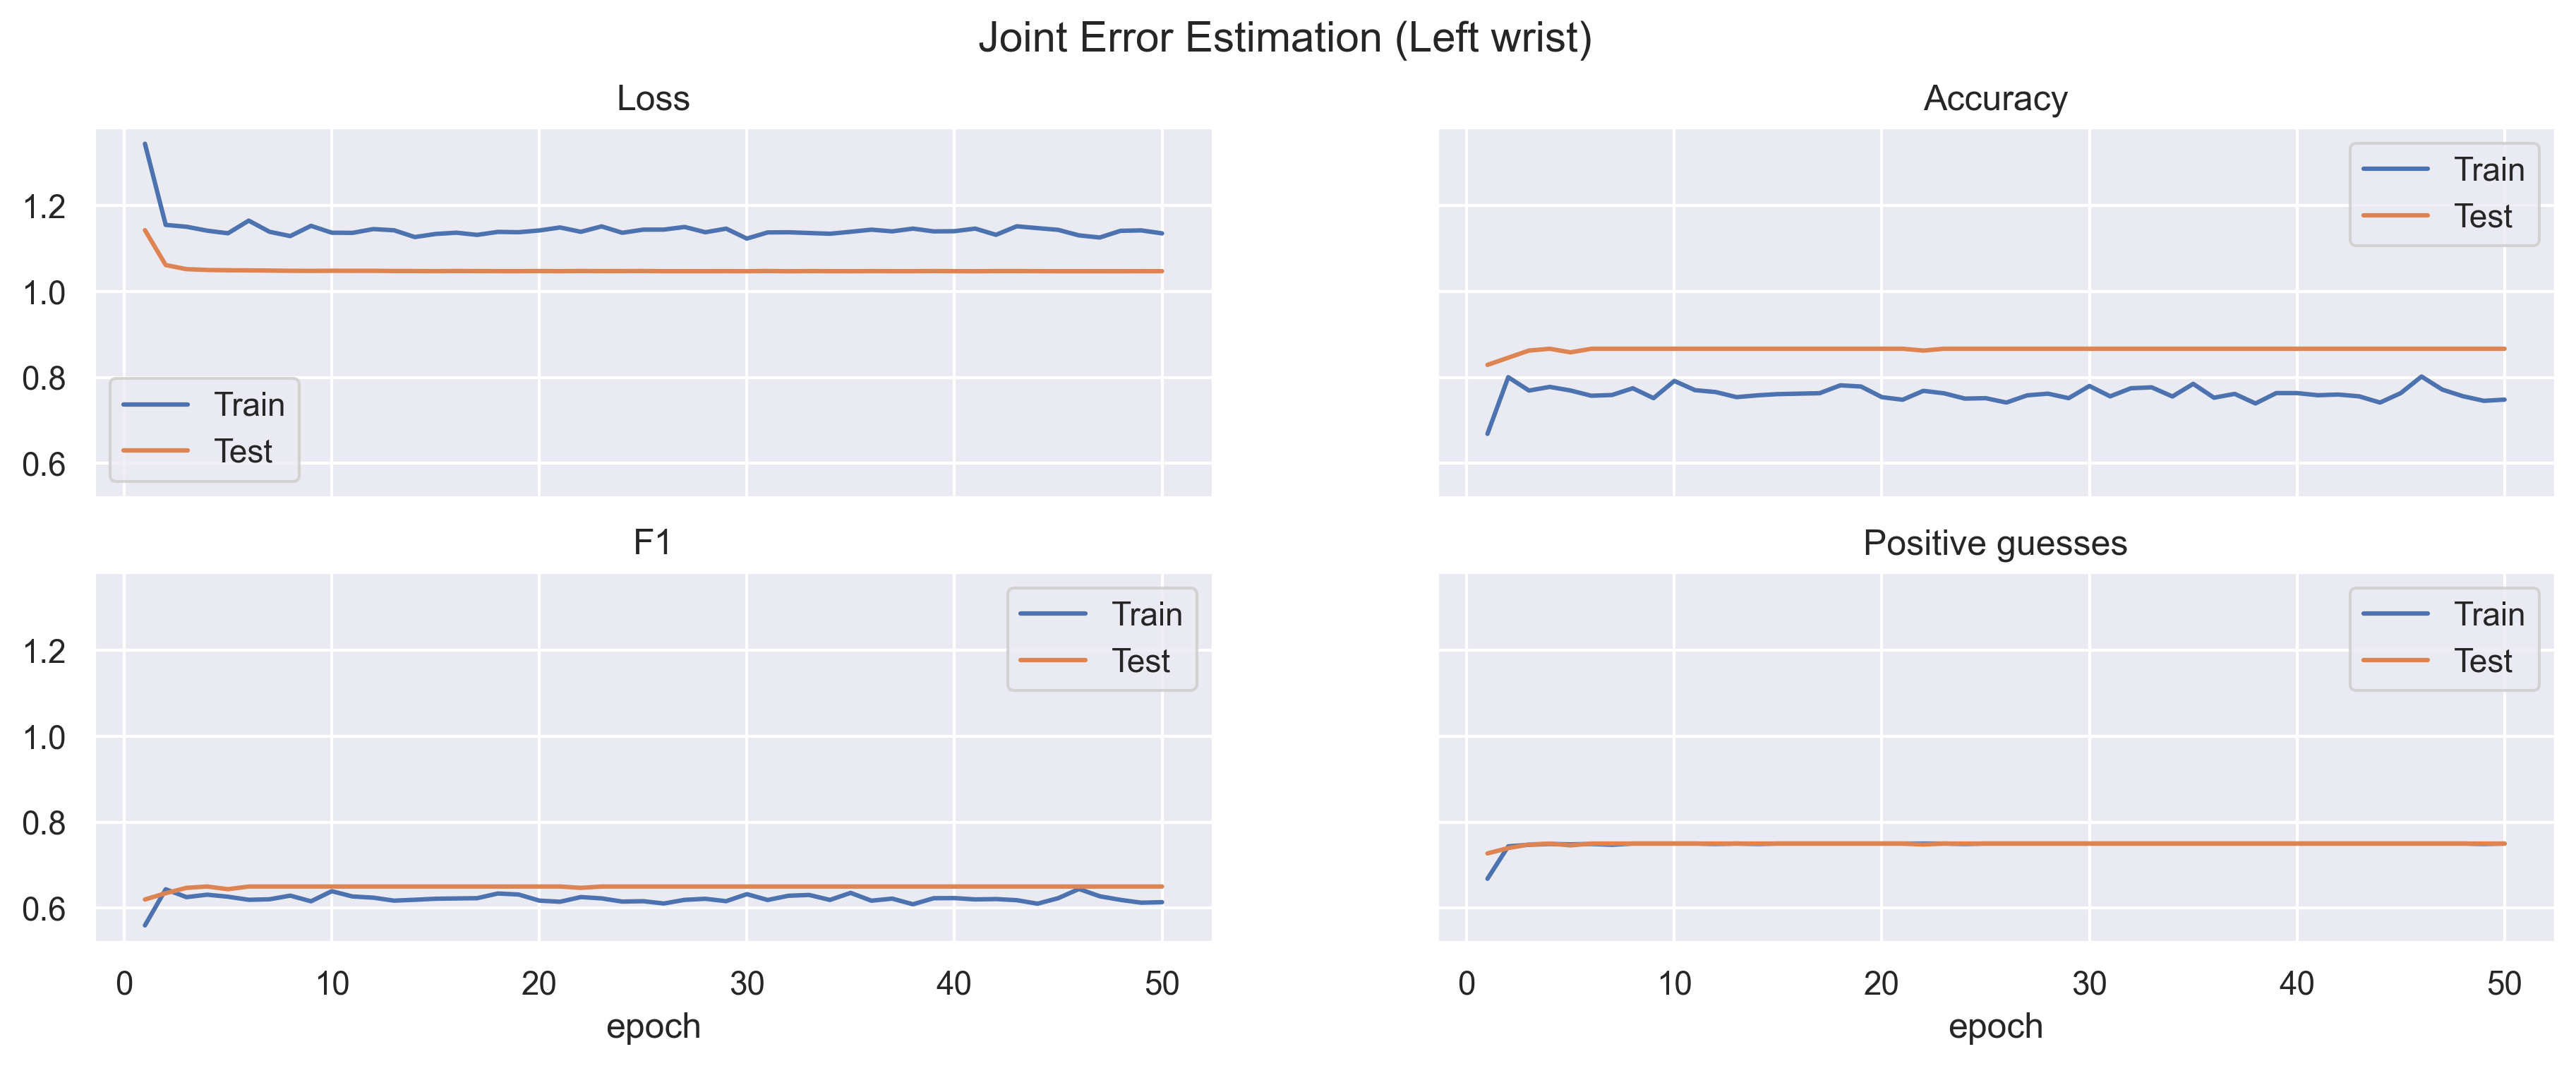
\includegraphics[width=\textwidth]{figures/Results/v1/jt/Left wrist_ErrorEstimation.png}
      \caption{Left Wrist Error Estimation}
      \label{fig:v1_lewr_jt_ee}
  \end{subfigure}
  \hfill
  \begin{subfigure}[b]{0.47\linewidth}
      \centering
      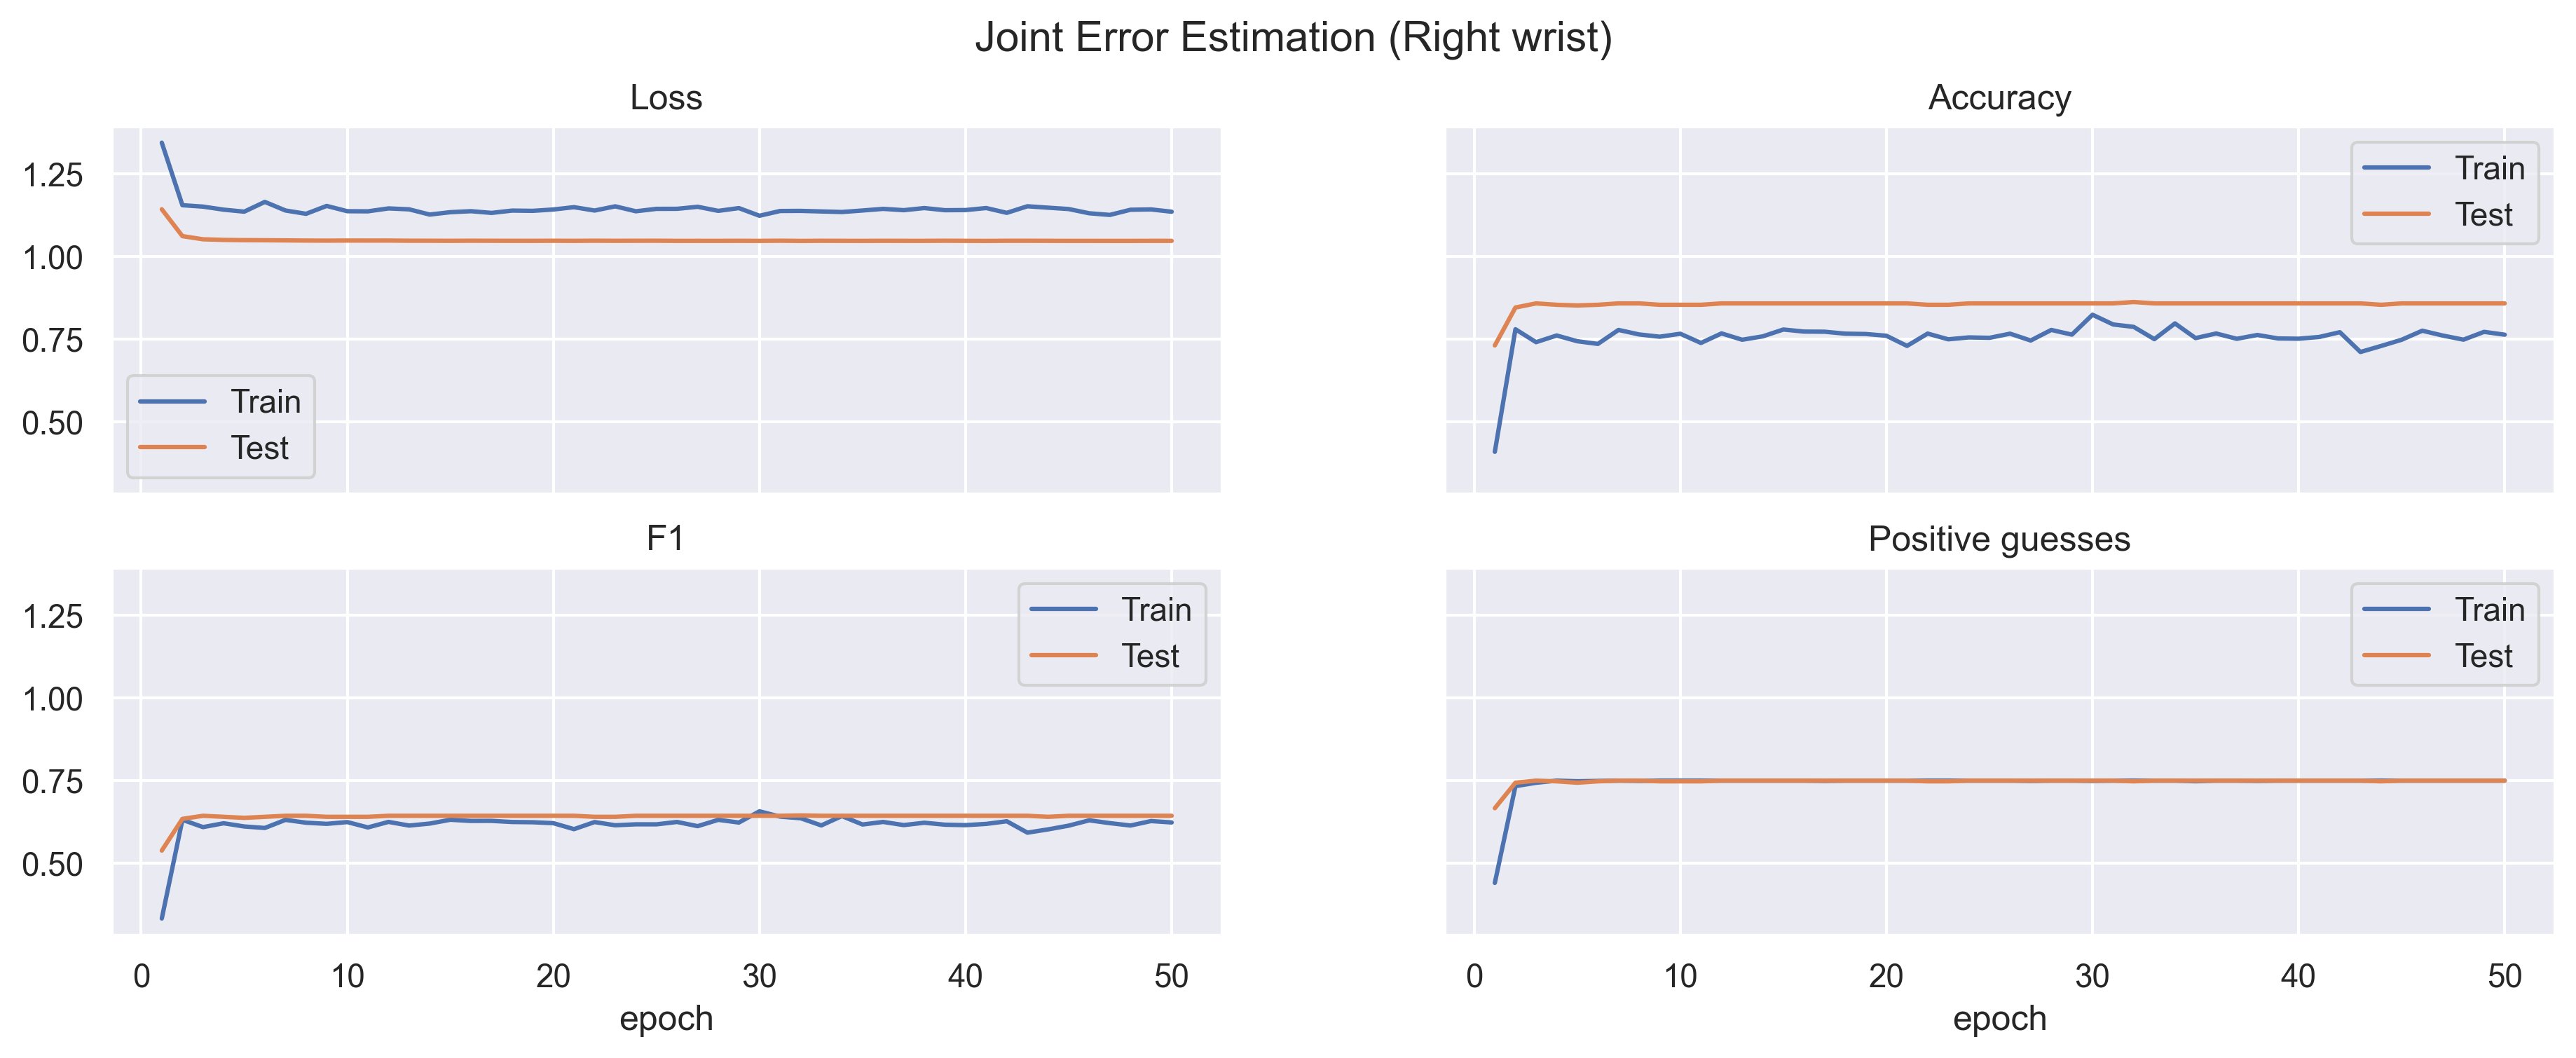
\includegraphics[width=\textwidth]{figures/Results/v1/jt/Right wrist_ErrorEstimation.png}
      \caption{Right Wrist Error Estimation}
      \label{fig:v1_riwr_jt_ee}
  \end{subfigure}
  \hfill
  \begin{subfigure}[b]{0.47\linewidth}
      \centering
      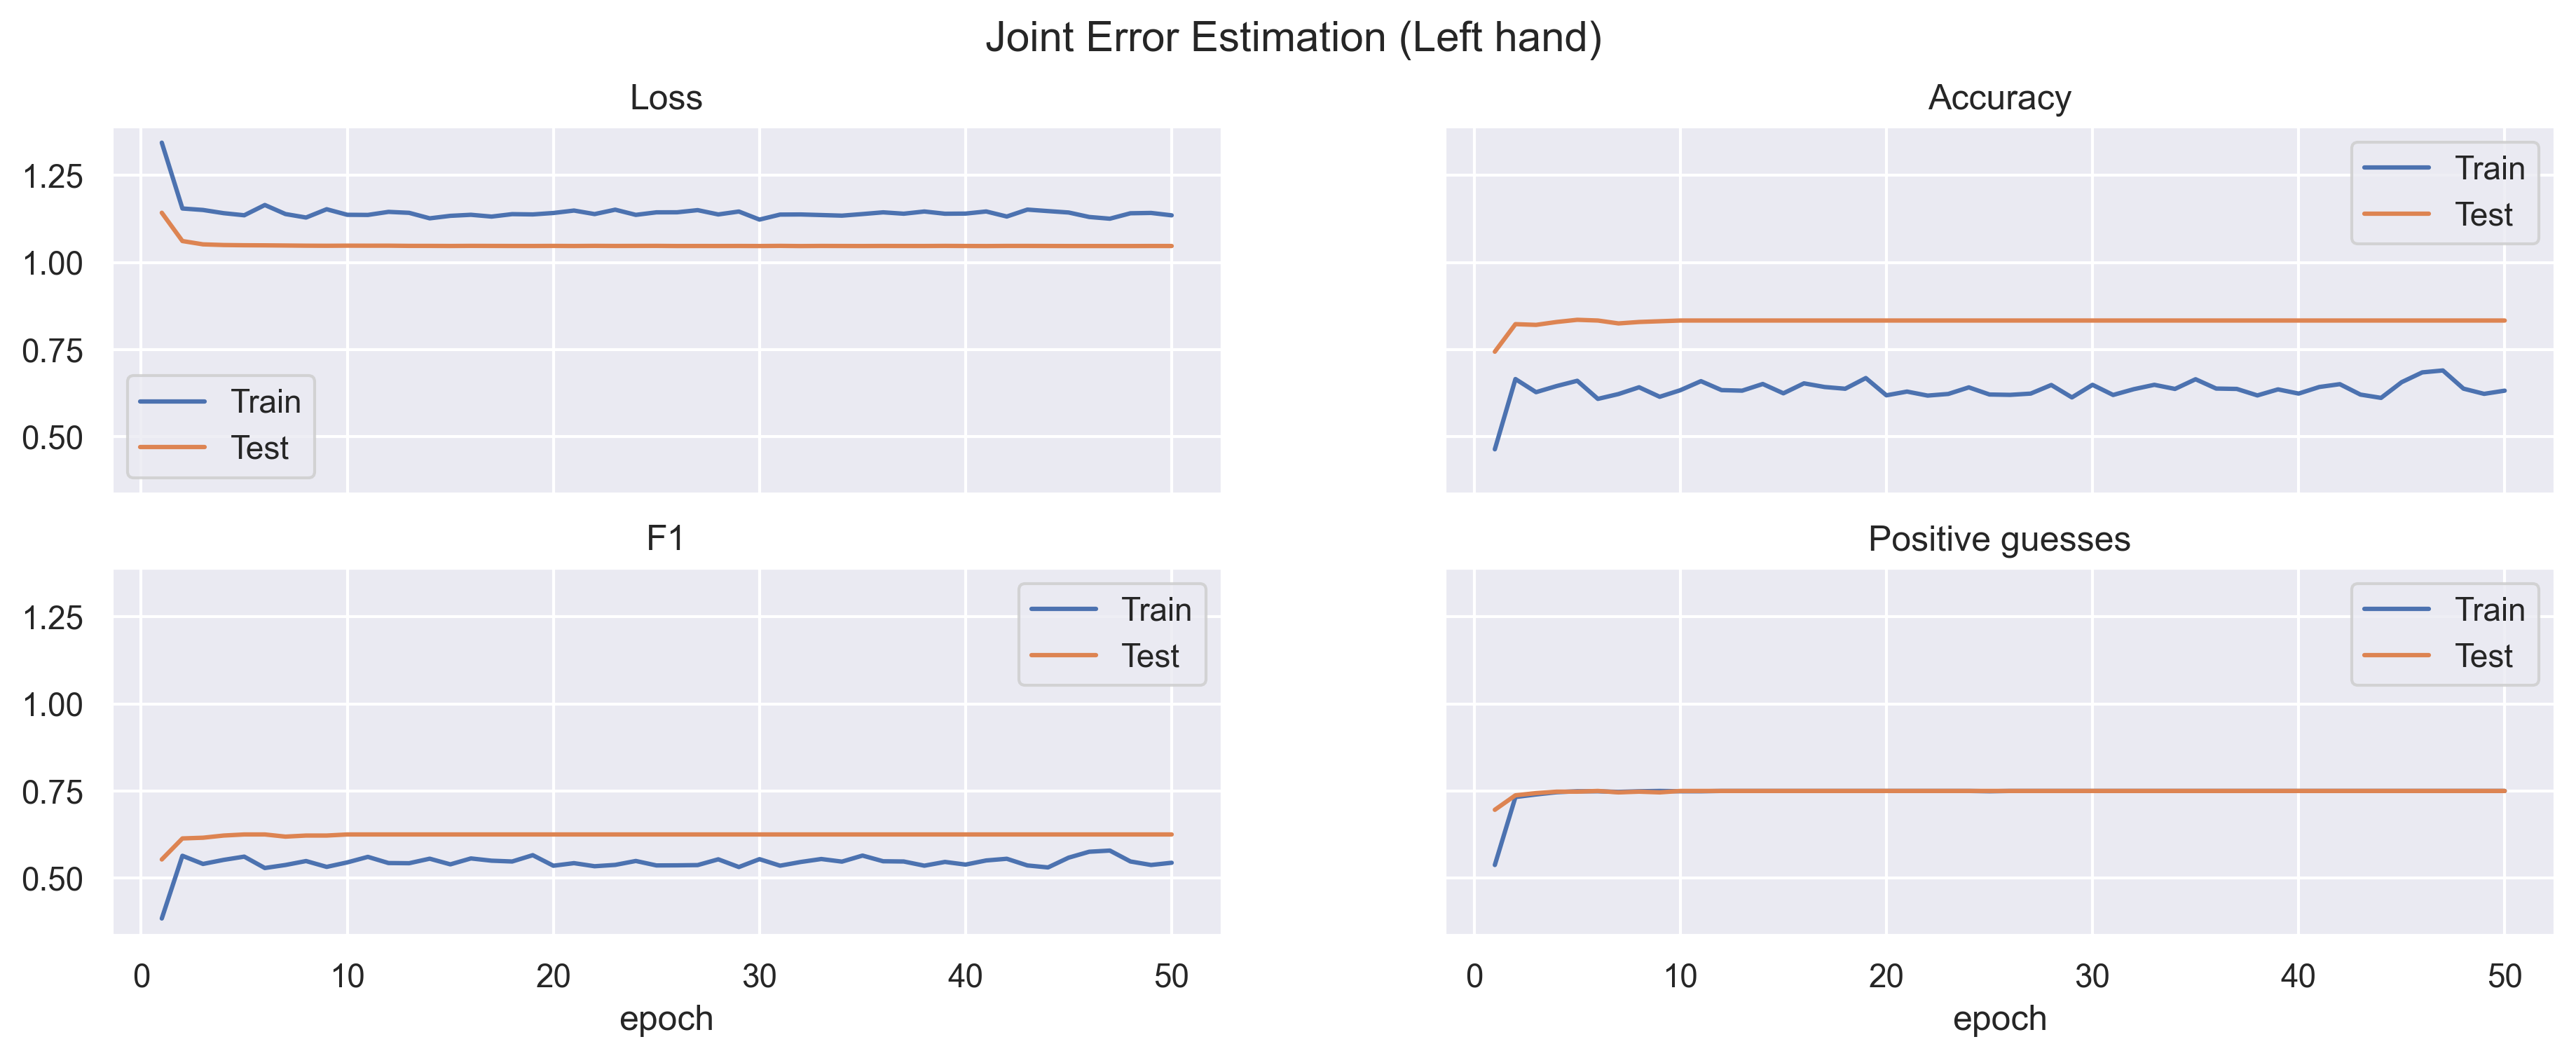
\includegraphics[width=\textwidth]{figures/Results/v1/jt/Left hand_ErrorEstimation.png}
      \caption{Left Hand Error Estimation}
      \label{fig:v1_leha_jt_ee}
  \end{subfigure}
  \hfill
  \begin{subfigure}[b]{0.47\linewidth}
      \centering
      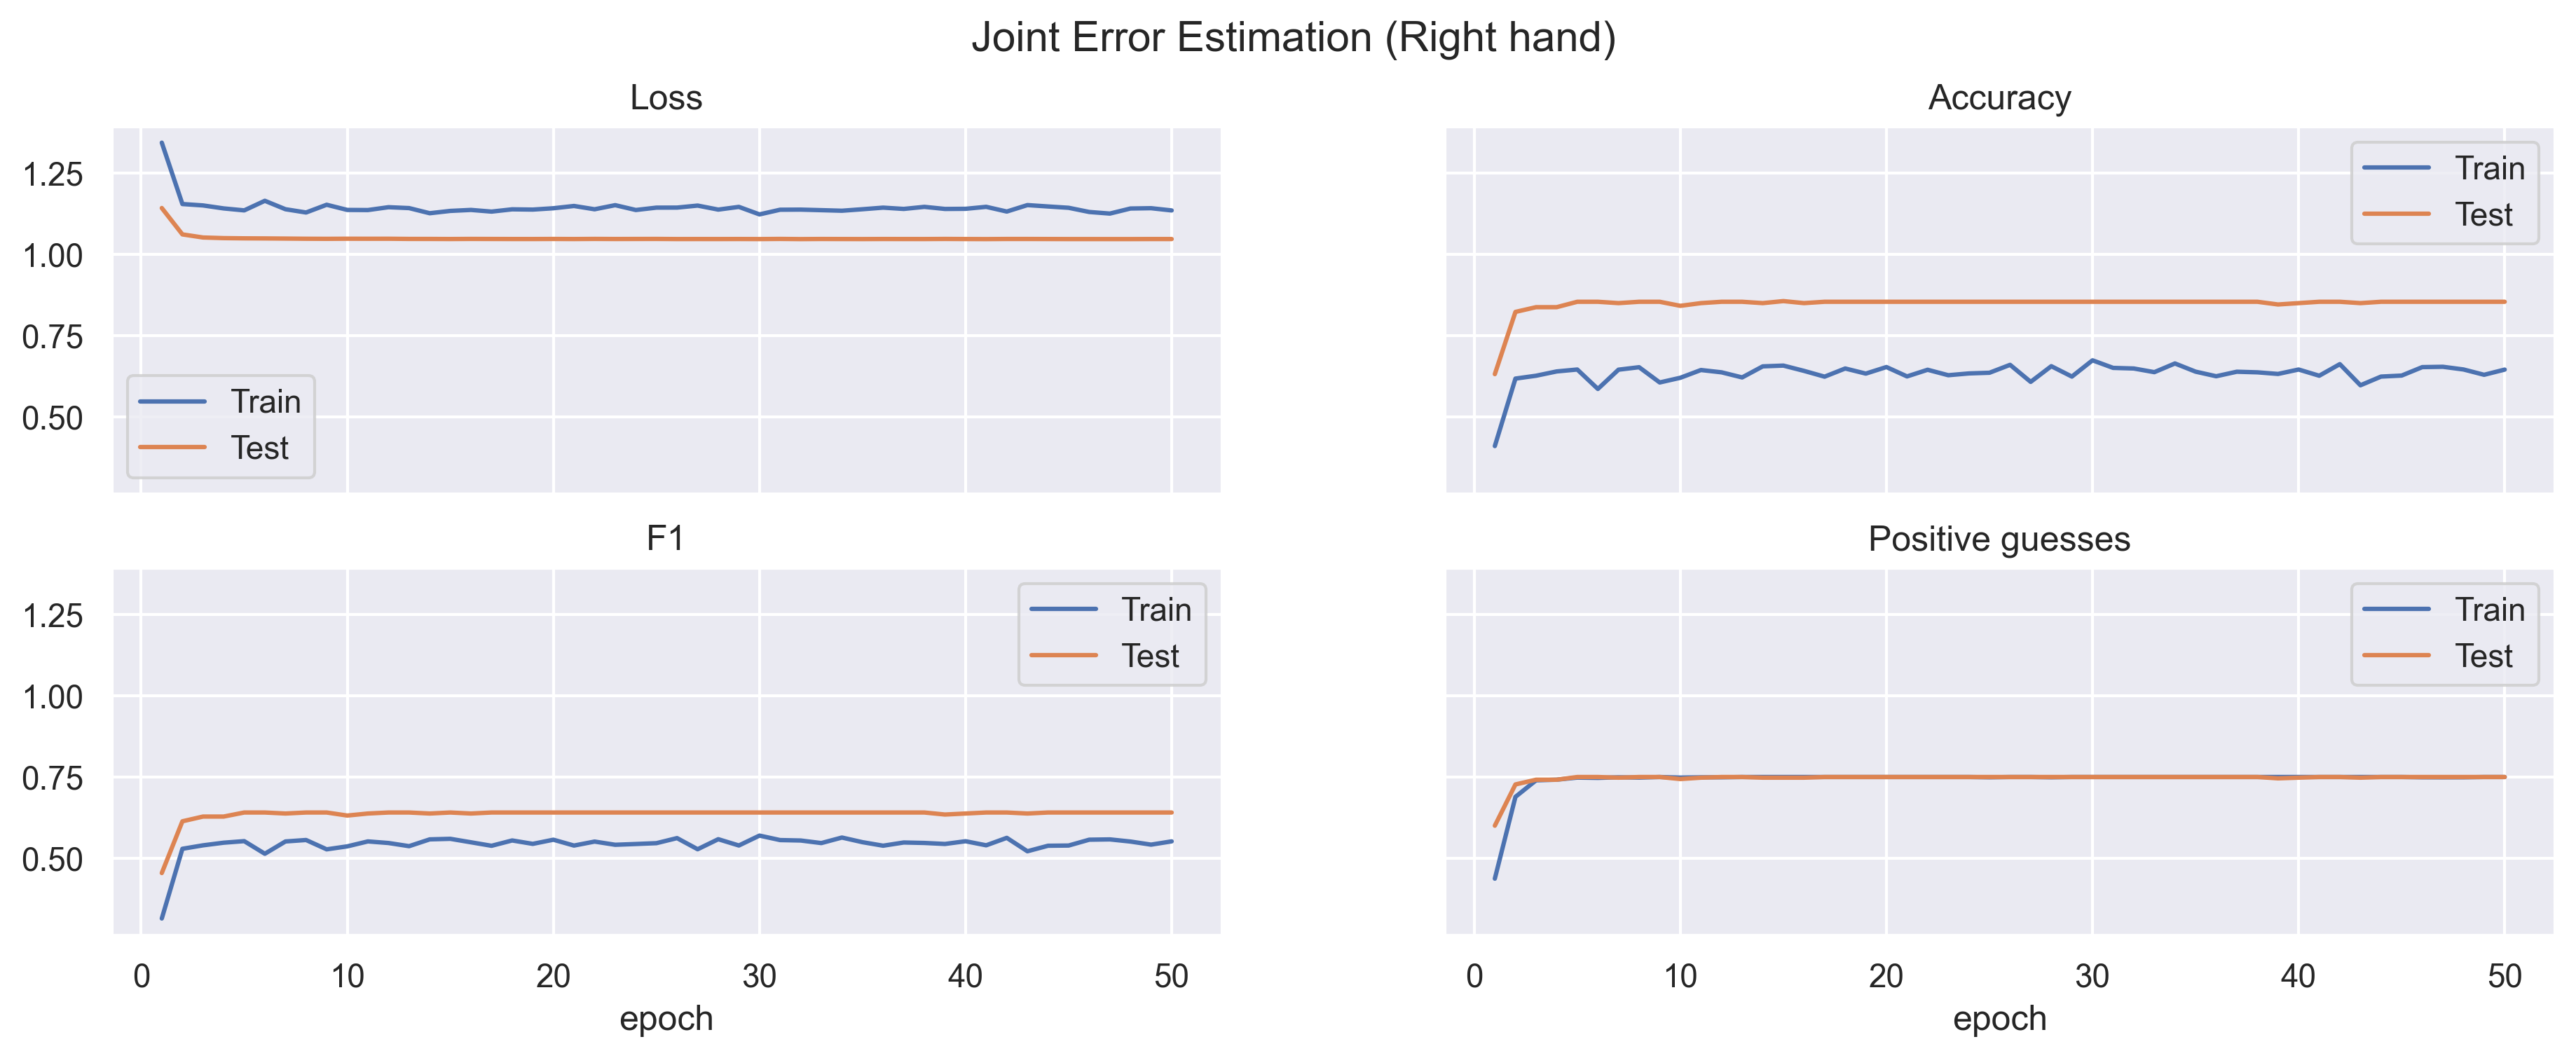
\includegraphics[width=\textwidth]{figures/Results/v1/jt/Right hand_ErrorEstimation.png}
      \caption{Left Arm Error Estimation}
      \label{fig:v1_riha_jt_ee}
  \end{subfigure}
\end{figure}

\begin{figure}[!htbp]
  \centering
  \begin{subfigure}[b]{0.47\linewidth}
      \centering
      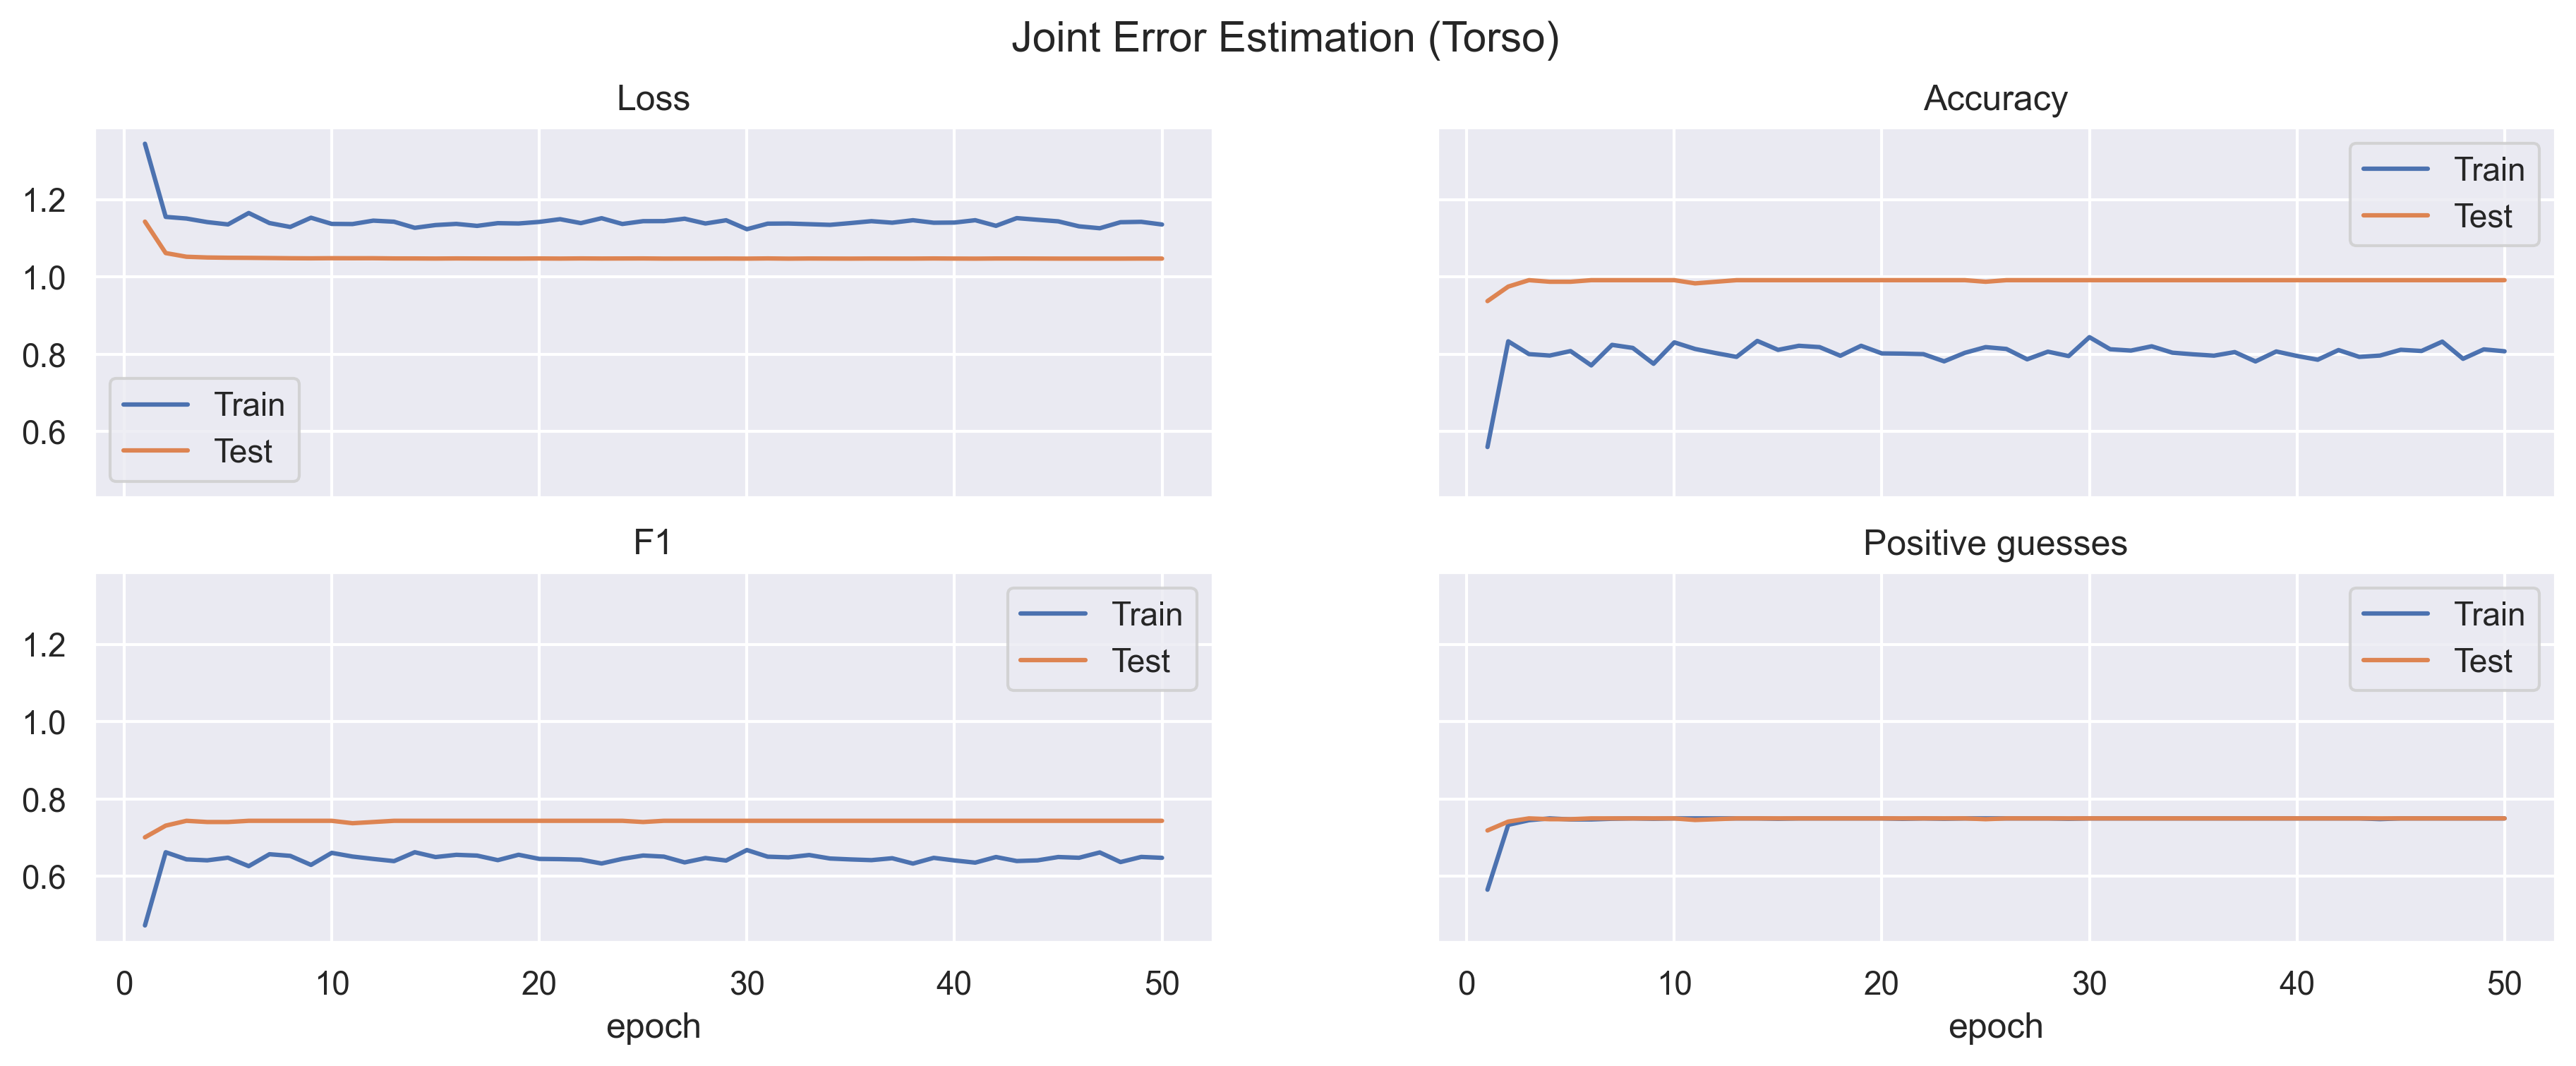
\includegraphics[width=\textwidth]{figures/Results/v1/jt/Torso_ErrorEstimation.png}
      \caption{Torso Error Estimation}
      \label{fig:v1_torso_jt_ee}
  \end{subfigure}
  \hfill
  \begin{subfigure}[b]{0.47\linewidth}
    \centering
    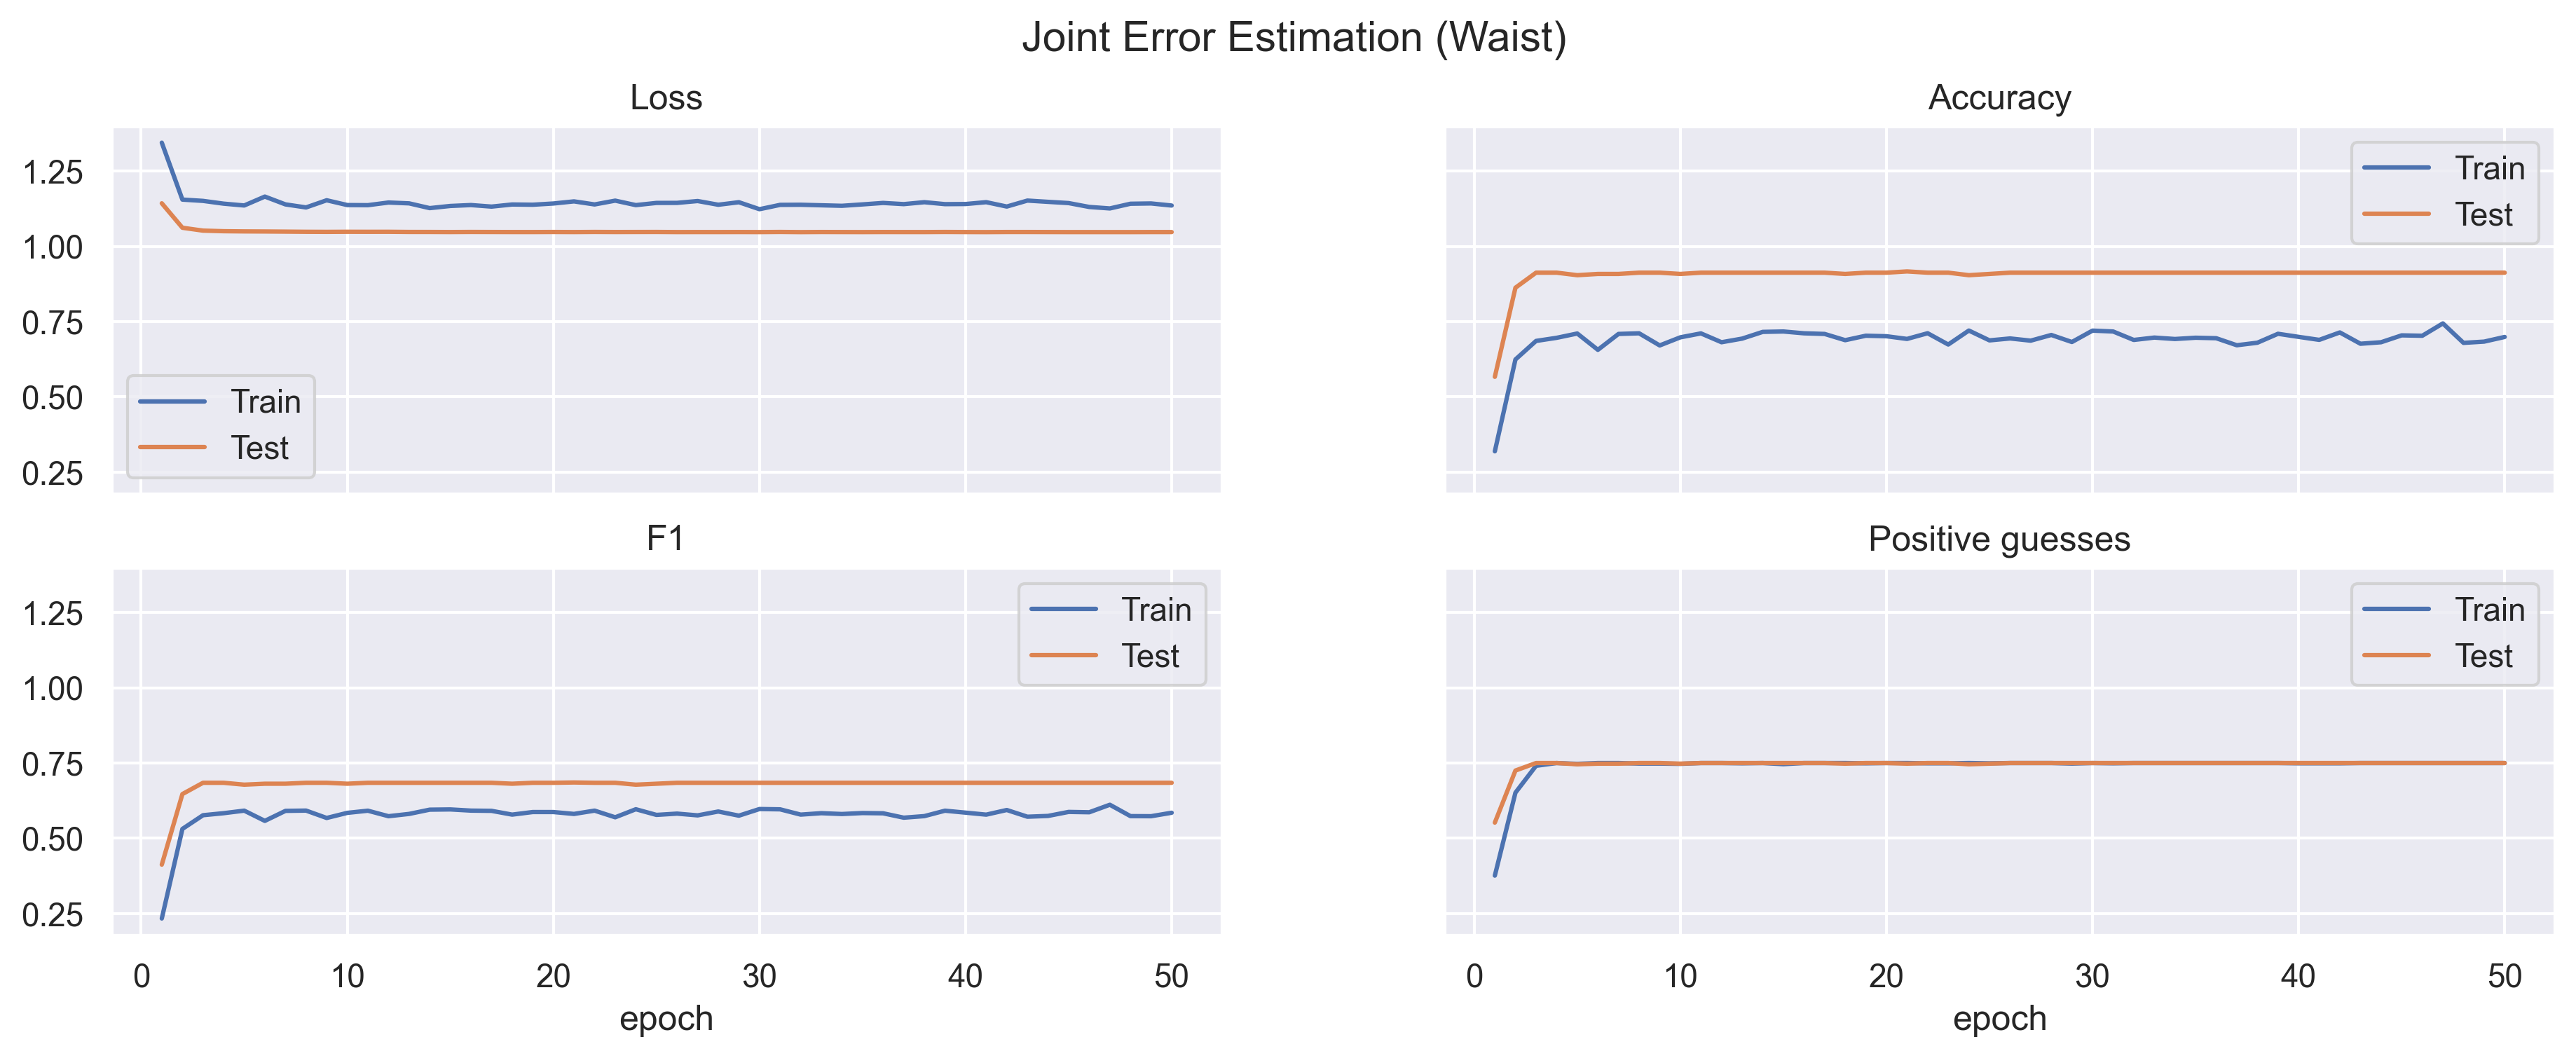
\includegraphics[width=\textwidth]{figures/Results/v1/jt/Waist_ErrorEstimation.png}
    \caption{Waist Error Estimation}
    \label{fig:v1_waist_jt_ee}
  \end{subfigure}
  \hfill
  \begin{subfigure}[b]{0.47\linewidth}
      \centering
      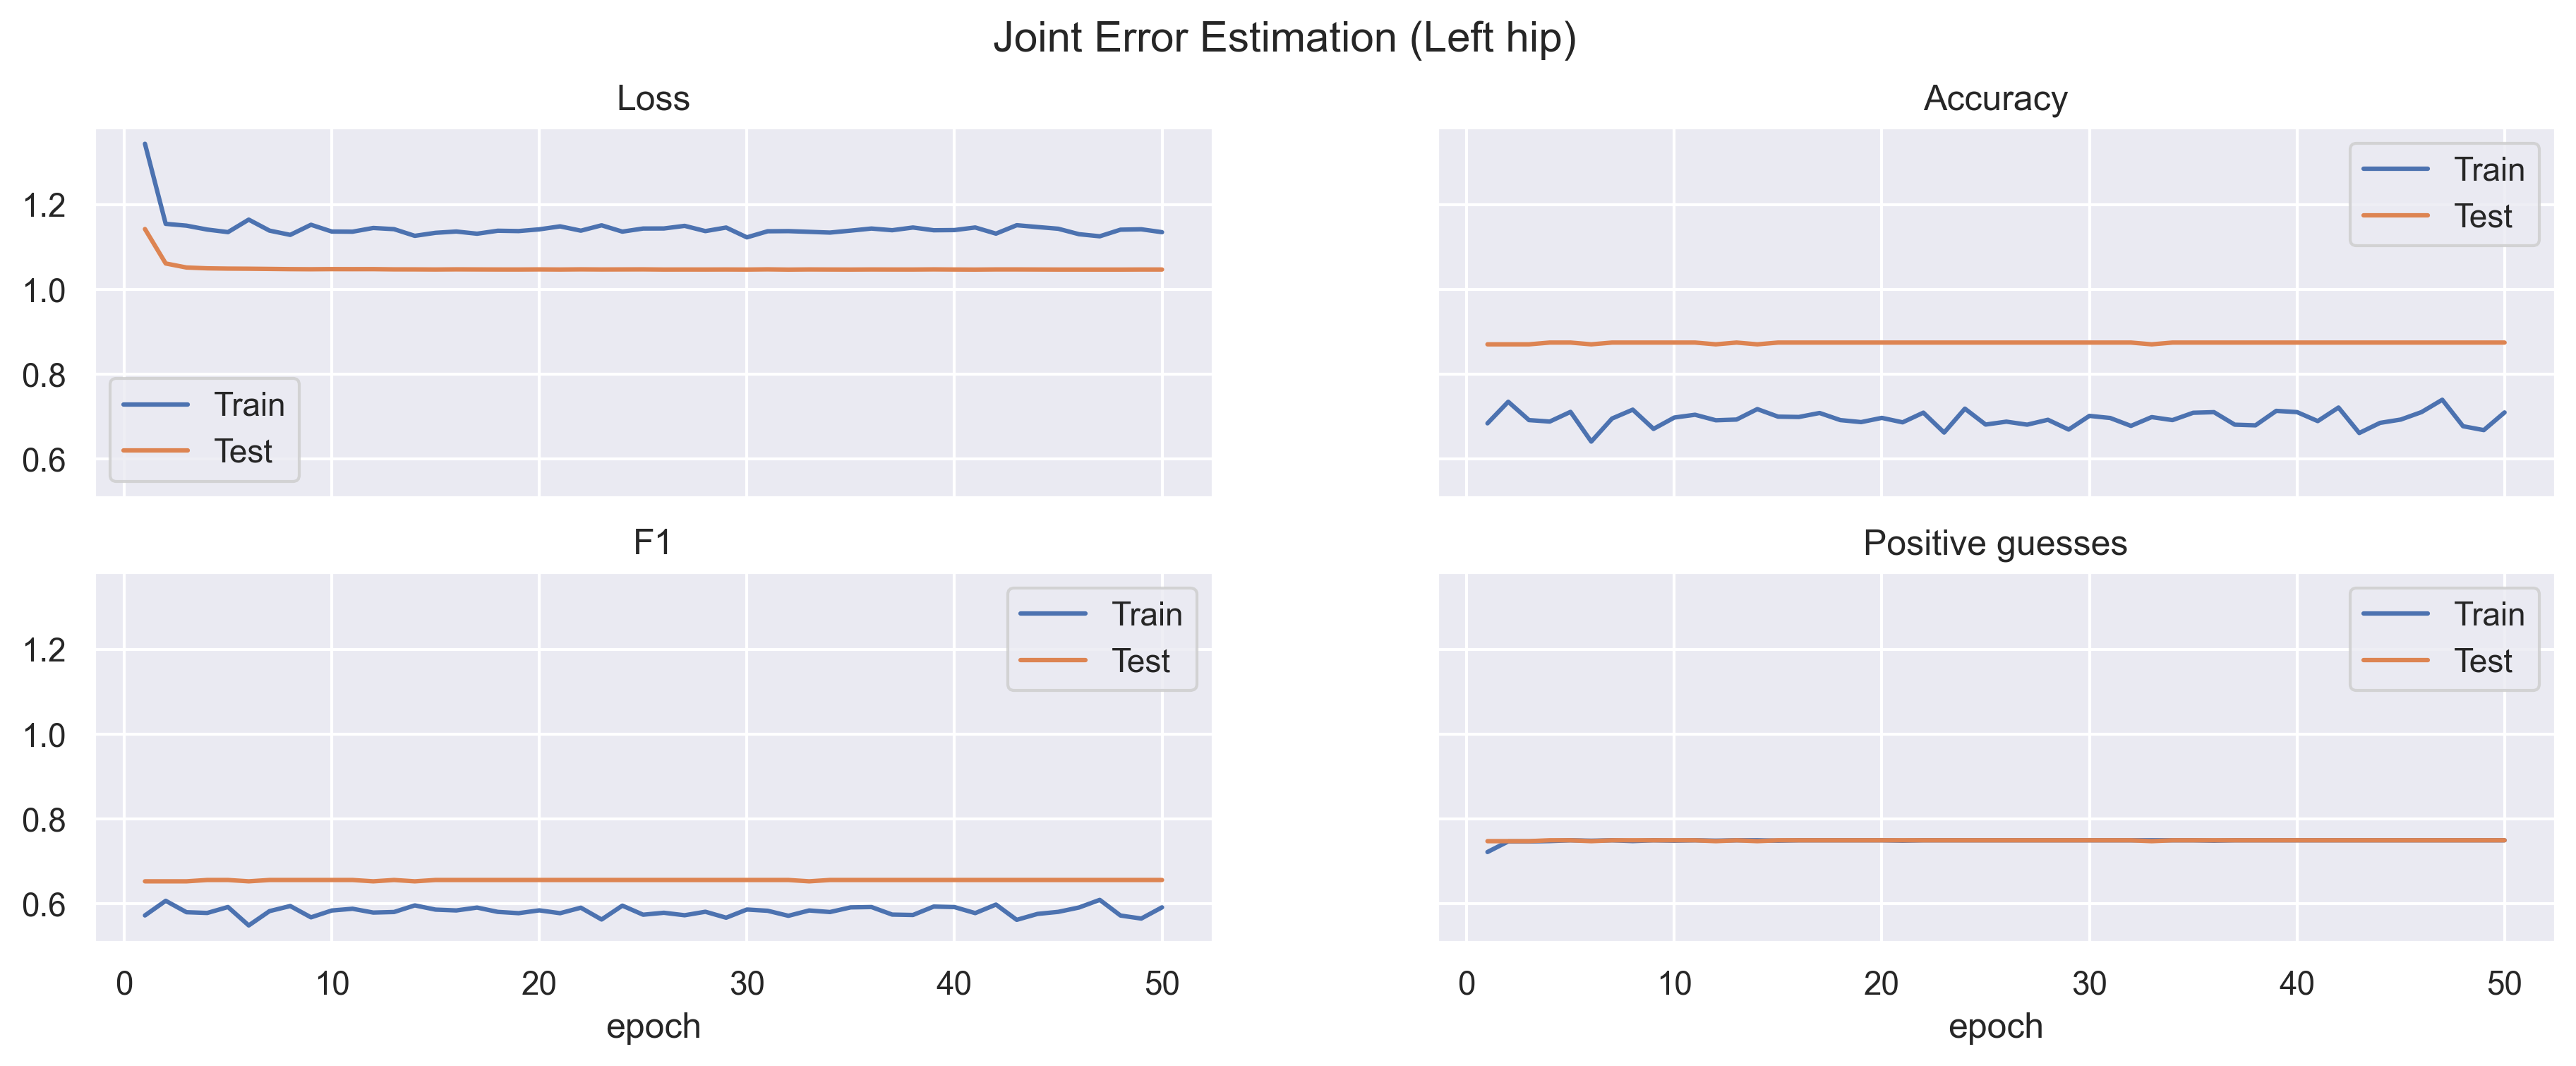
\includegraphics[width=\textwidth]{figures/Results/v1/jt/Left hip_ErrorEstimation.png}
      \caption{Left Hip Error Estimation}
      \label{fig:v1_lehi_jt_ee}
  \end{subfigure}
  \hfill
  \begin{subfigure}[b]{0.47\linewidth}
      \centering
      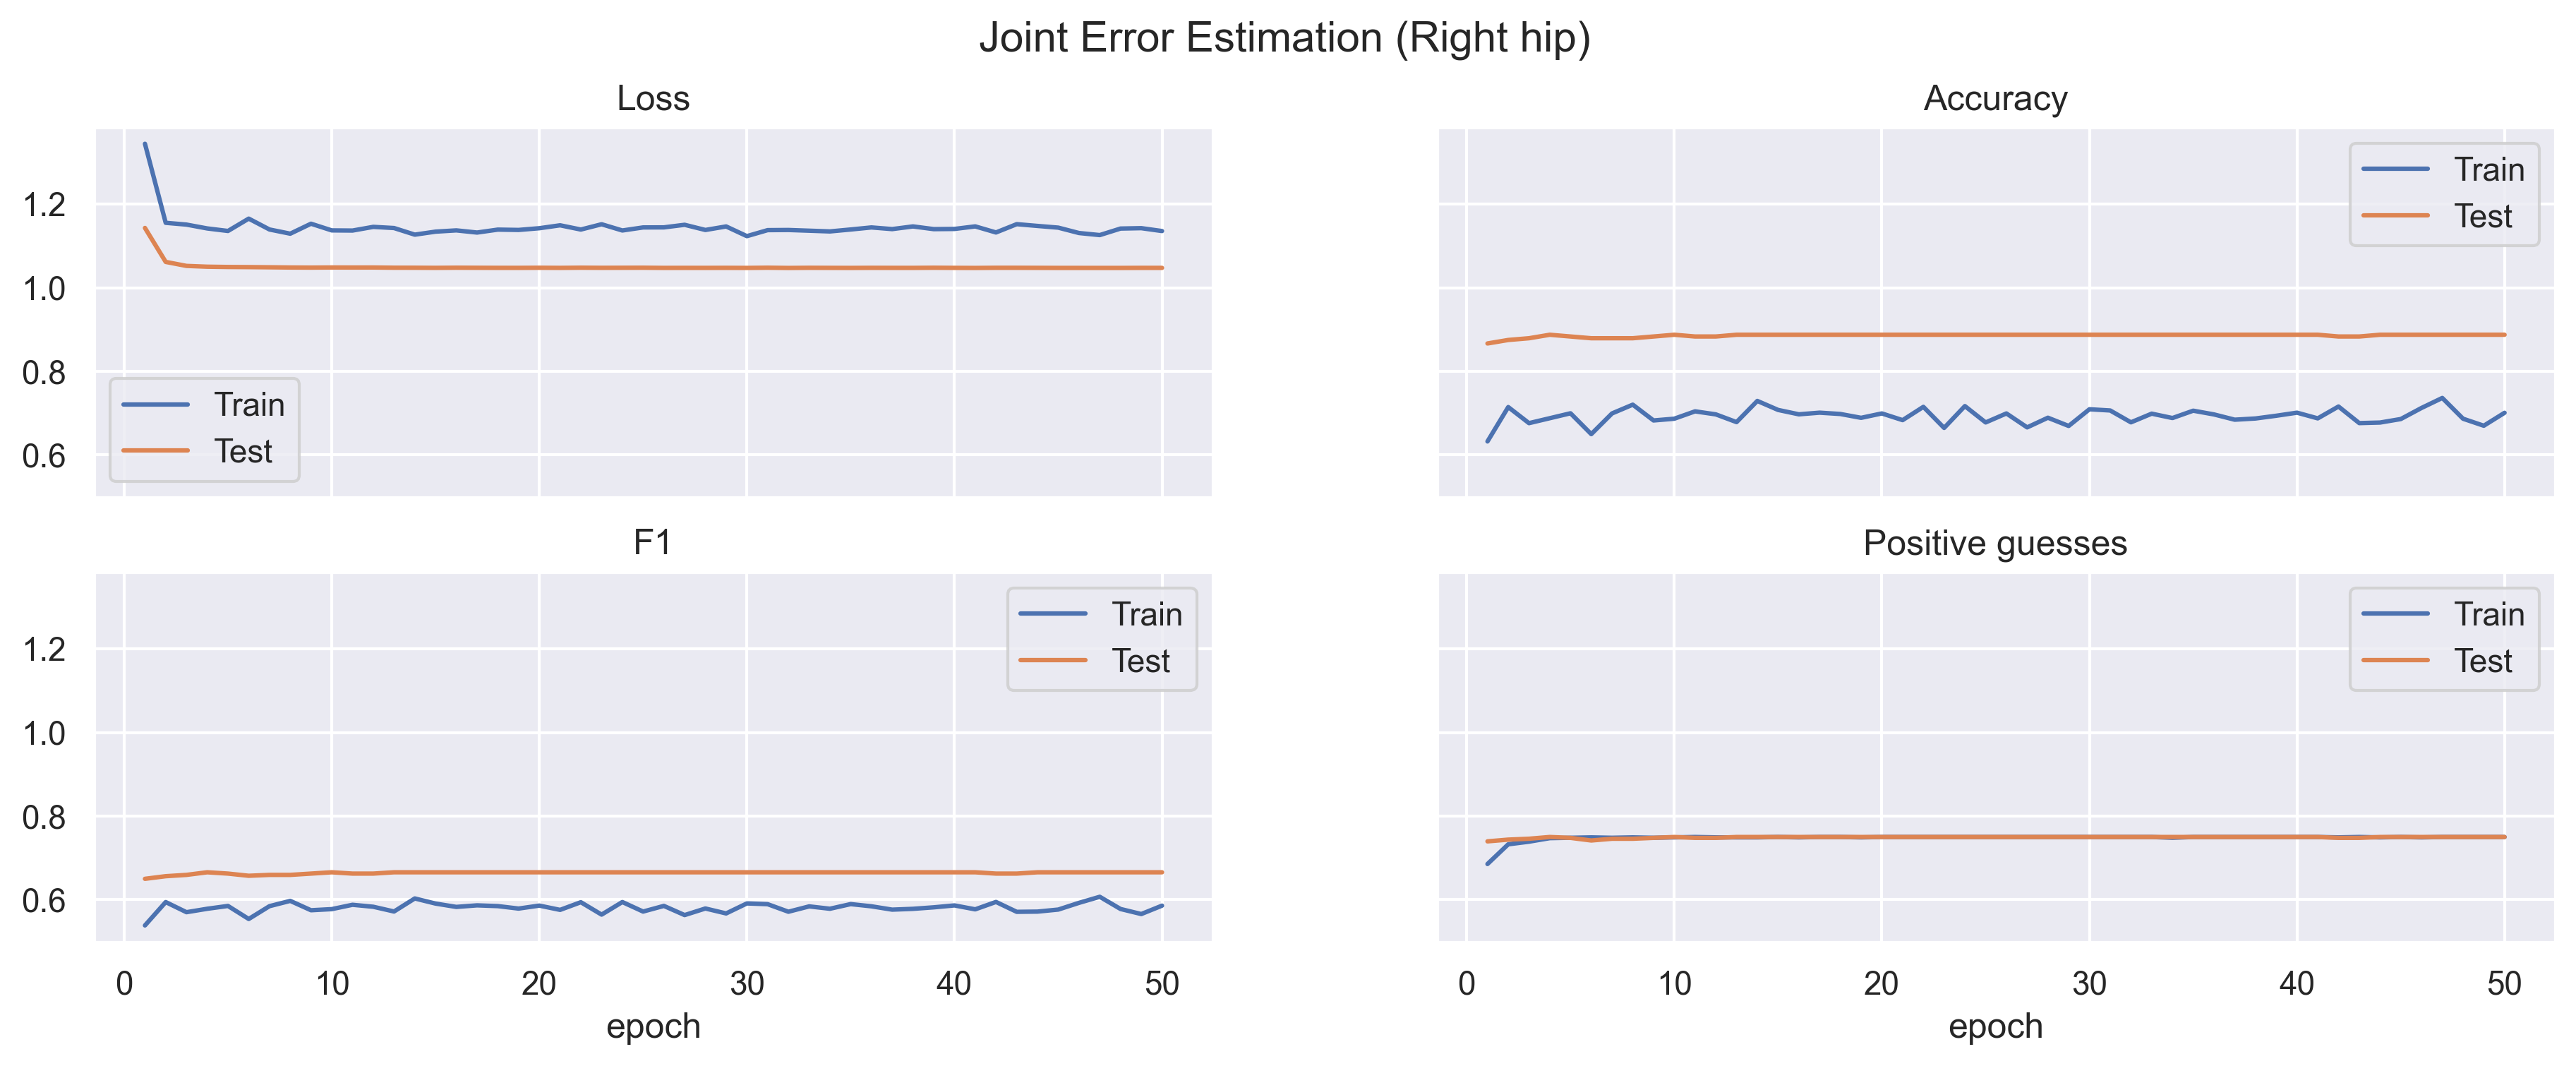
\includegraphics[width=\textwidth]{figures/Results/v1/jt/Right hip_ErrorEstimation.png}
      \caption{Right hip Error Estimation}
      \label{fig:v1_rihi_jt_ee}
  \end{subfigure}
\end{figure}


\begin{figure}[!htbp]
  \centering
  \begin{subfigure}[b]{0.47\linewidth}
      \centering
      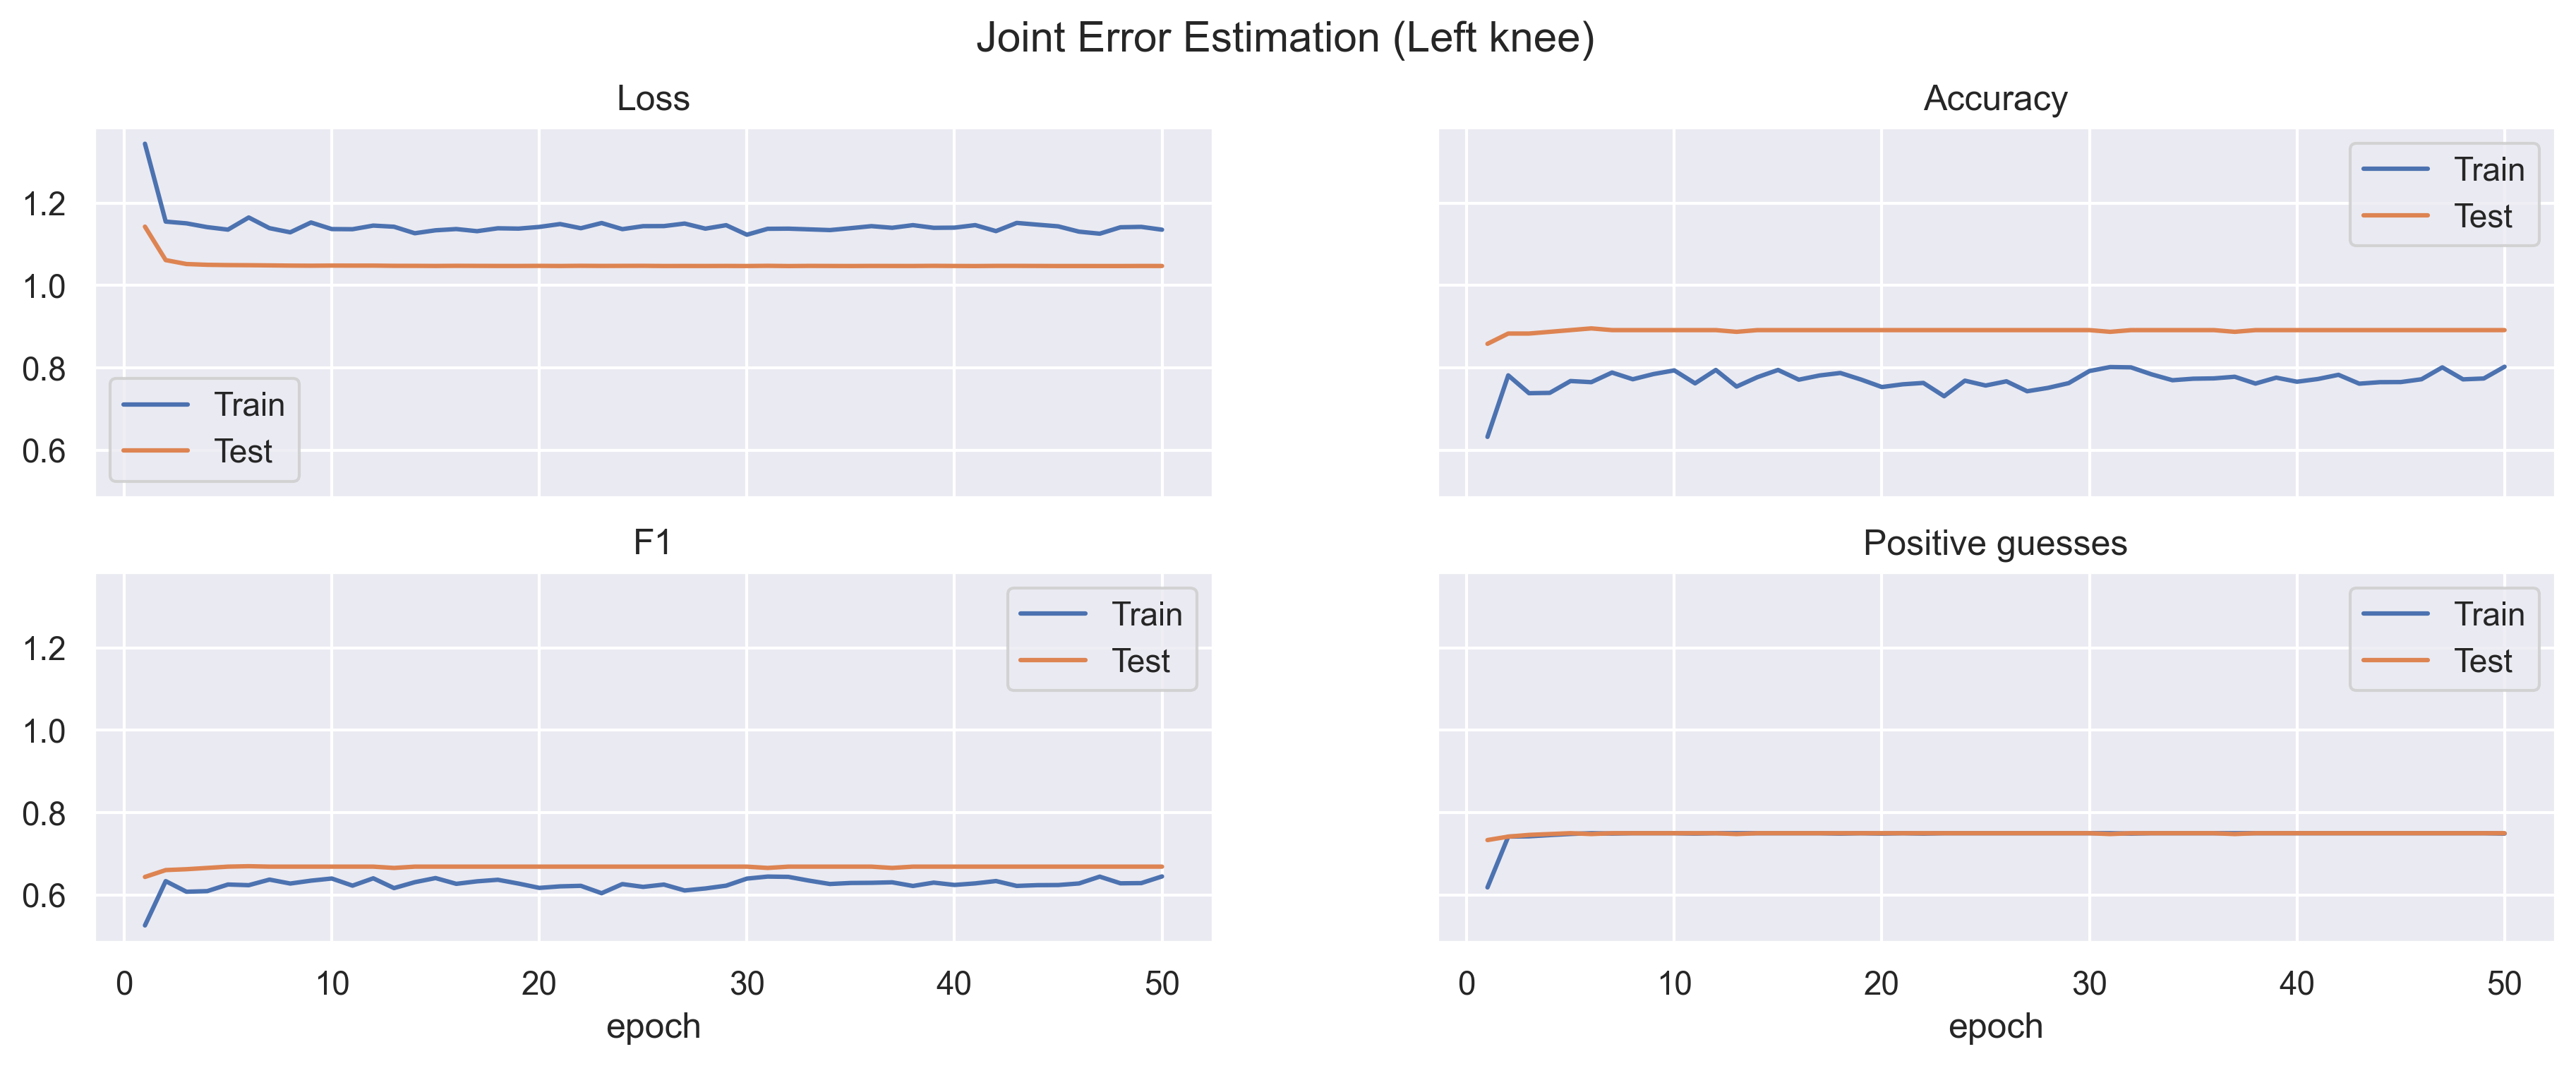
\includegraphics[width=\textwidth]{figures/Results/v1/jt/Left knee_ErrorEstimation.png}
      \caption{left Knee Error Estimation}
      \label{fig:v1_lekn_jt_ee}
  \end{subfigure}
  \hfill
  \begin{subfigure}[b]{0.47\linewidth}
      \centering
      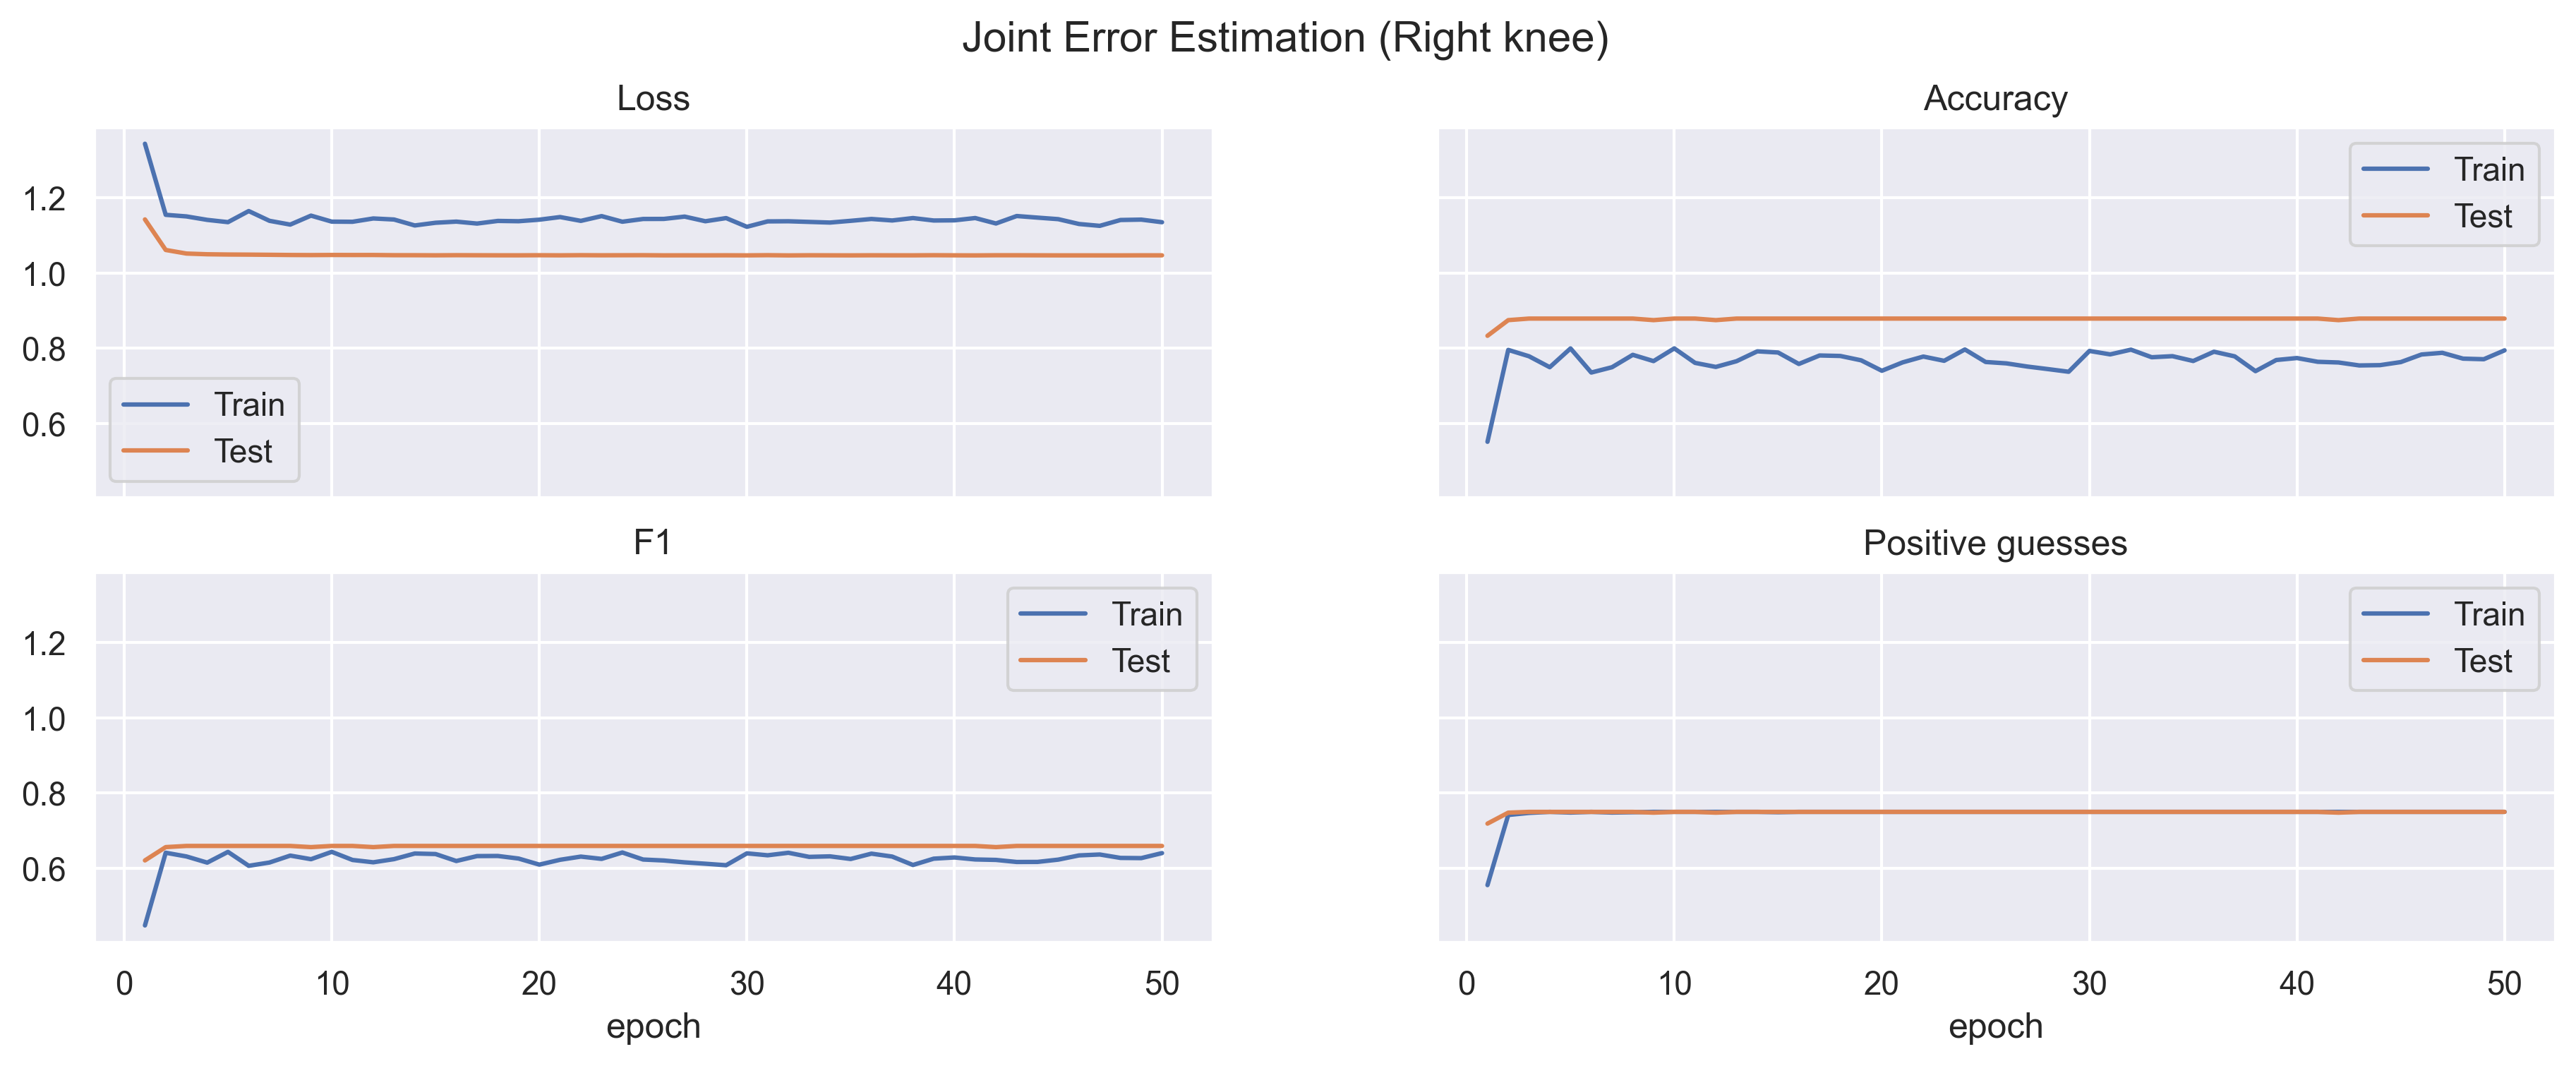
\includegraphics[width=\textwidth]{figures/Results/v1/jt/Right knee_ErrorEstimation.png}
      \caption{Right Knee Error Estimation}
      \label{fig:v1_rikn_jt_ee}
  \end{subfigure}
  \hfill
  \begin{subfigure}[b]{0.47\linewidth}
      \centering
      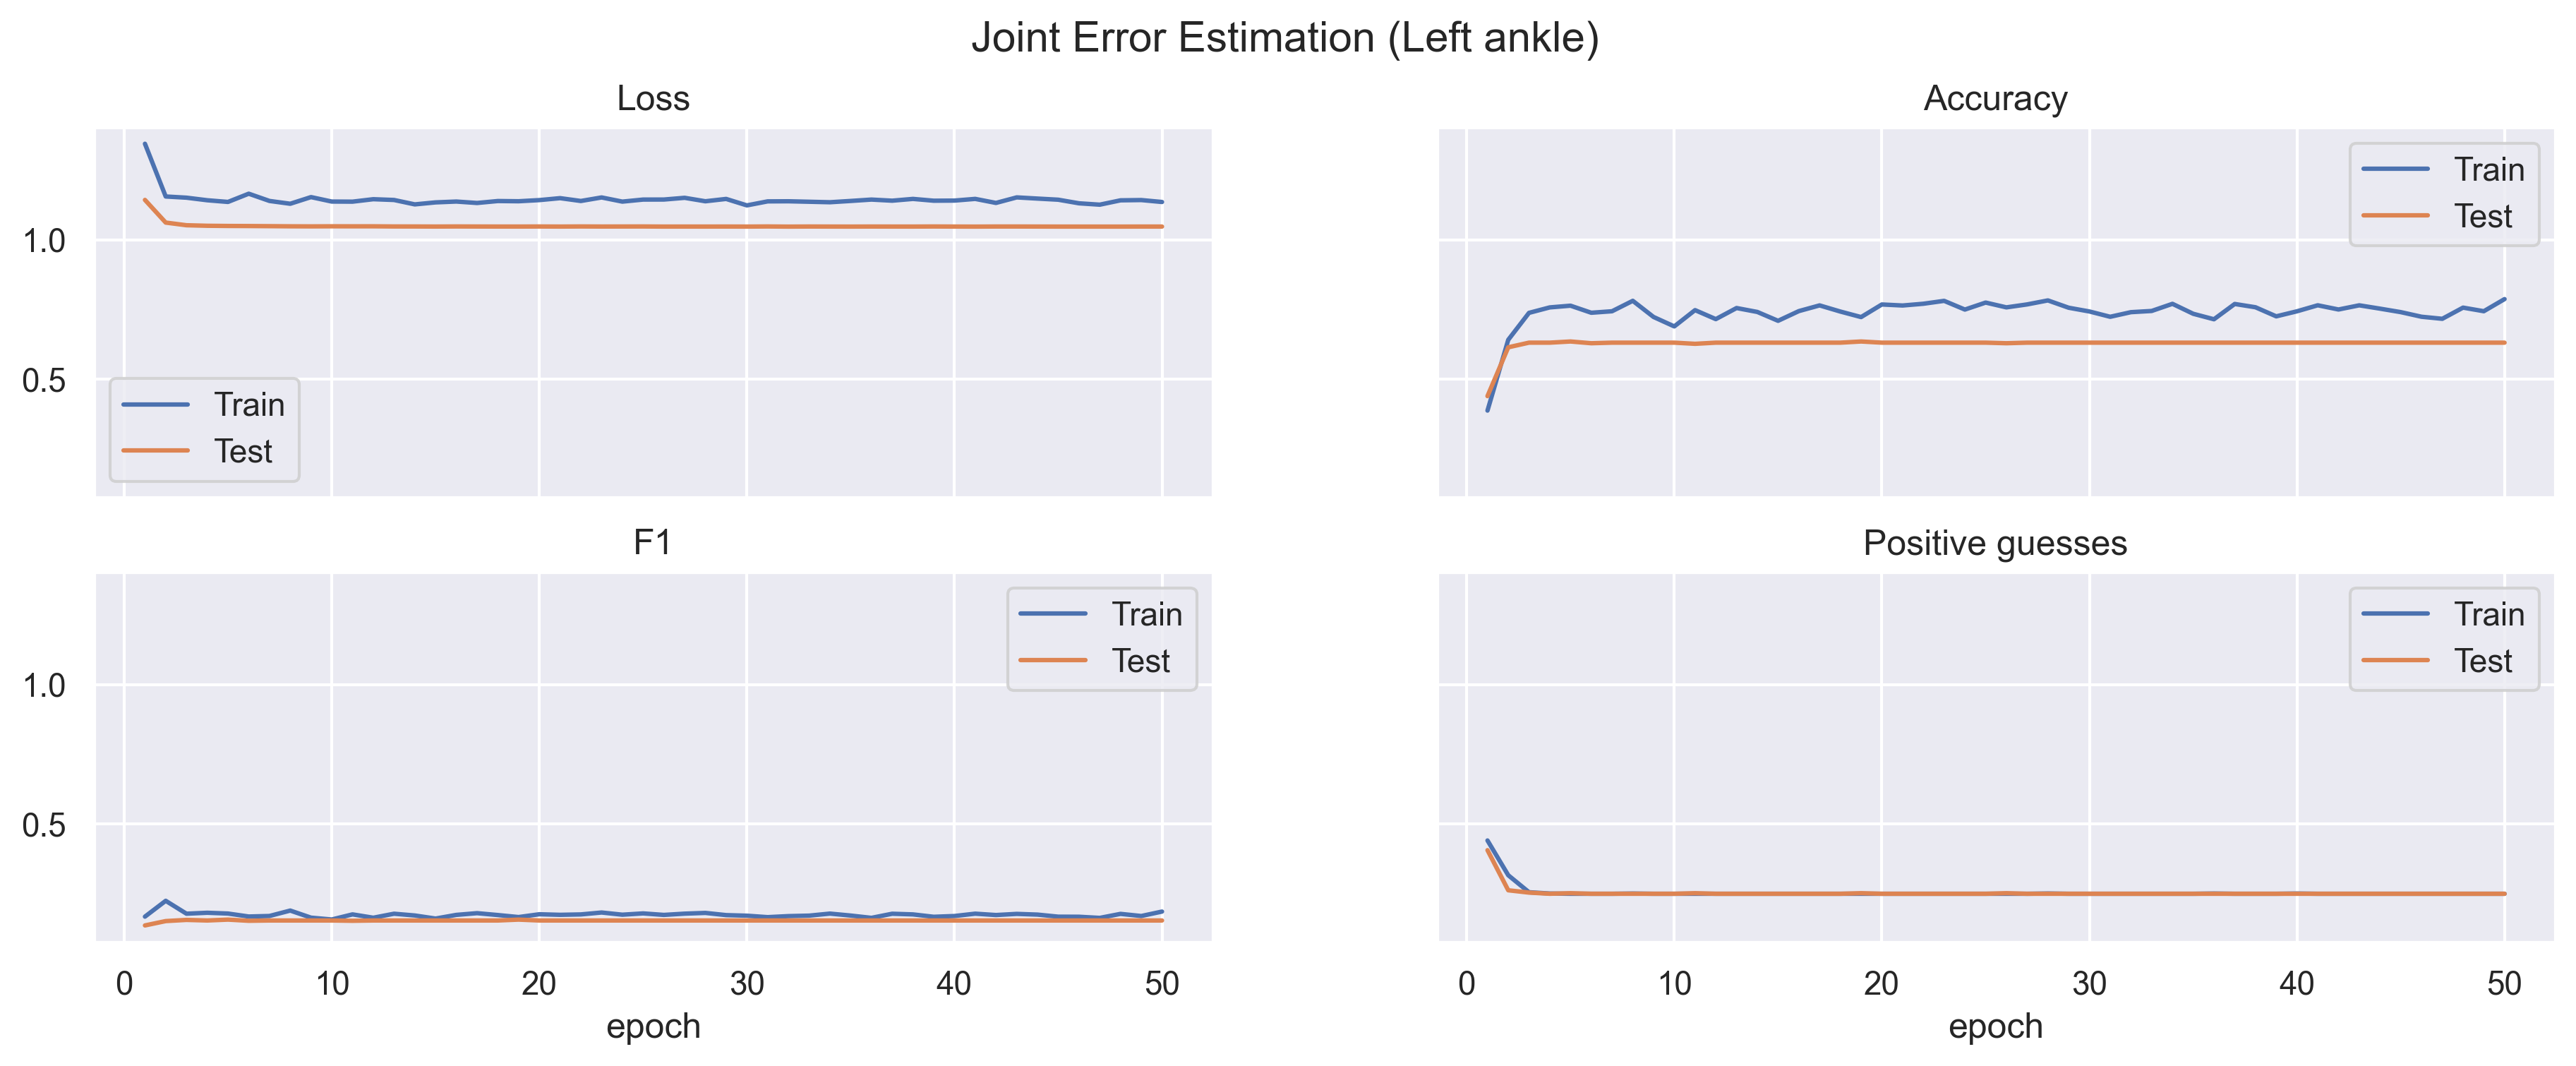
\includegraphics[width=\textwidth]{figures/Results/v1/jt/Left ankle_ErrorEstimation.png}
      \caption{Left Ankle Error Estimation}
      \label{fig:v1_lean_jt_ee}
  \end{subfigure}
  \hfill
  \begin{subfigure}[b]{0.47\linewidth}
      \centering
      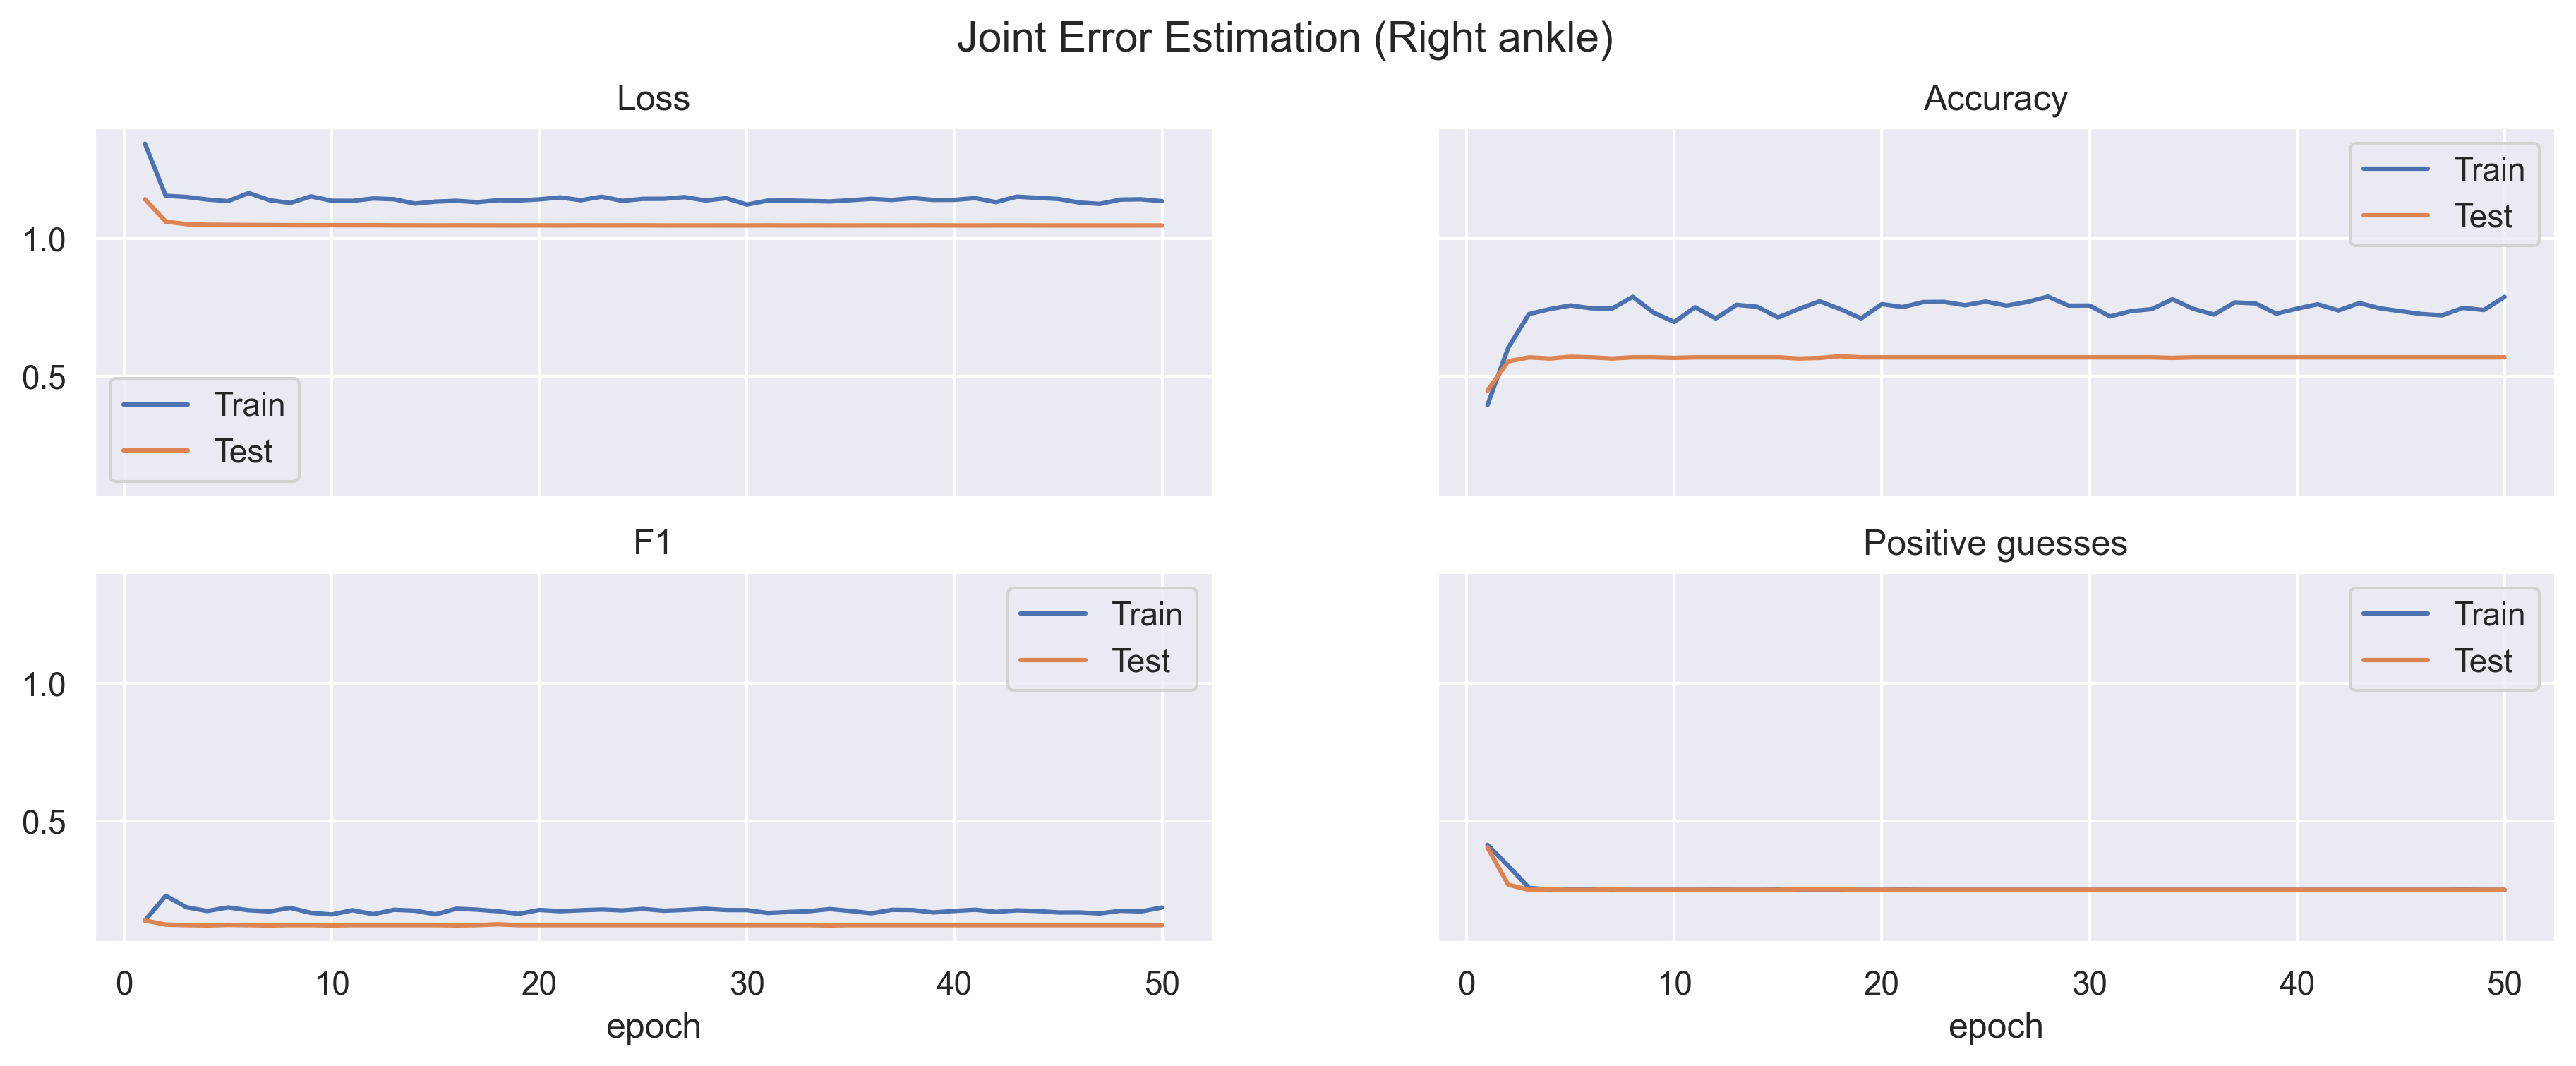
\includegraphics[width=\textwidth]{figures/Results/v1/jt/Right ankle_ErrorEstimation.png}
      \caption{Right Ankle Error Estimation}
      \label{fig:v1_rian_jt_ee}
  \end{subfigure}
  \caption[Detailed Training results for the Joint Problem Set]{The training results of the Joint error estimation model for FESDModelv1.}
  \label{fig:joint_training_results}
\end{figure}